\section{Results and Discussion}
\label{ch1:sec:results-and-discussion}

In this section, the results are outlined that were generated from all simulations. In each of the three subsections, the performances of the AIMD and AIMD+ algorithm are compared against each other. To do so, the performance metrics outlined in Section \ref{ch1:subsec:performance-metric-definition} were used. In the following subsections, results from the four test cases defined as {A}, {B}, {C} and {D} in Section \ref{ch1:subsec:test-cases-and-scenarios} are explained first, then the results from the full analysis over the large range of EV and battery storage uptake is presented. In the end, these results are summarised and discussed.

\subsection{Voltage Violation Analysis}

For the comparison of voltage improvements, results compared the algorithms' performances at reducing bus voltage variation; particularly by increasing the lowest recorded bus voltage. Each load's bus voltage was recorded, from which a sample voltage profile, Figure \ref{ch1:fig:voltage-profiles-excerpt}, was extracted, where the bus voltage fluctuation over time becomes apparent. It can be seen that the introduction of EVs has significantly lowered the line-to-neutral voltage. Adding energy BESS devices did raise the voltage levels during times of peak demand, as can be seen between 17:00 and 21:00, where the AIMD+ algorithm has elevated voltages further than the AIMD scenario. To obtain a better understanding of the level of improvement, the voltage frequency distribution of all buses along the feeder was generated and plotted in a histogram in Figure \ref{ch1:fig:voltage-violation-excerpt}.

\begin{figure}[htb]\centering
	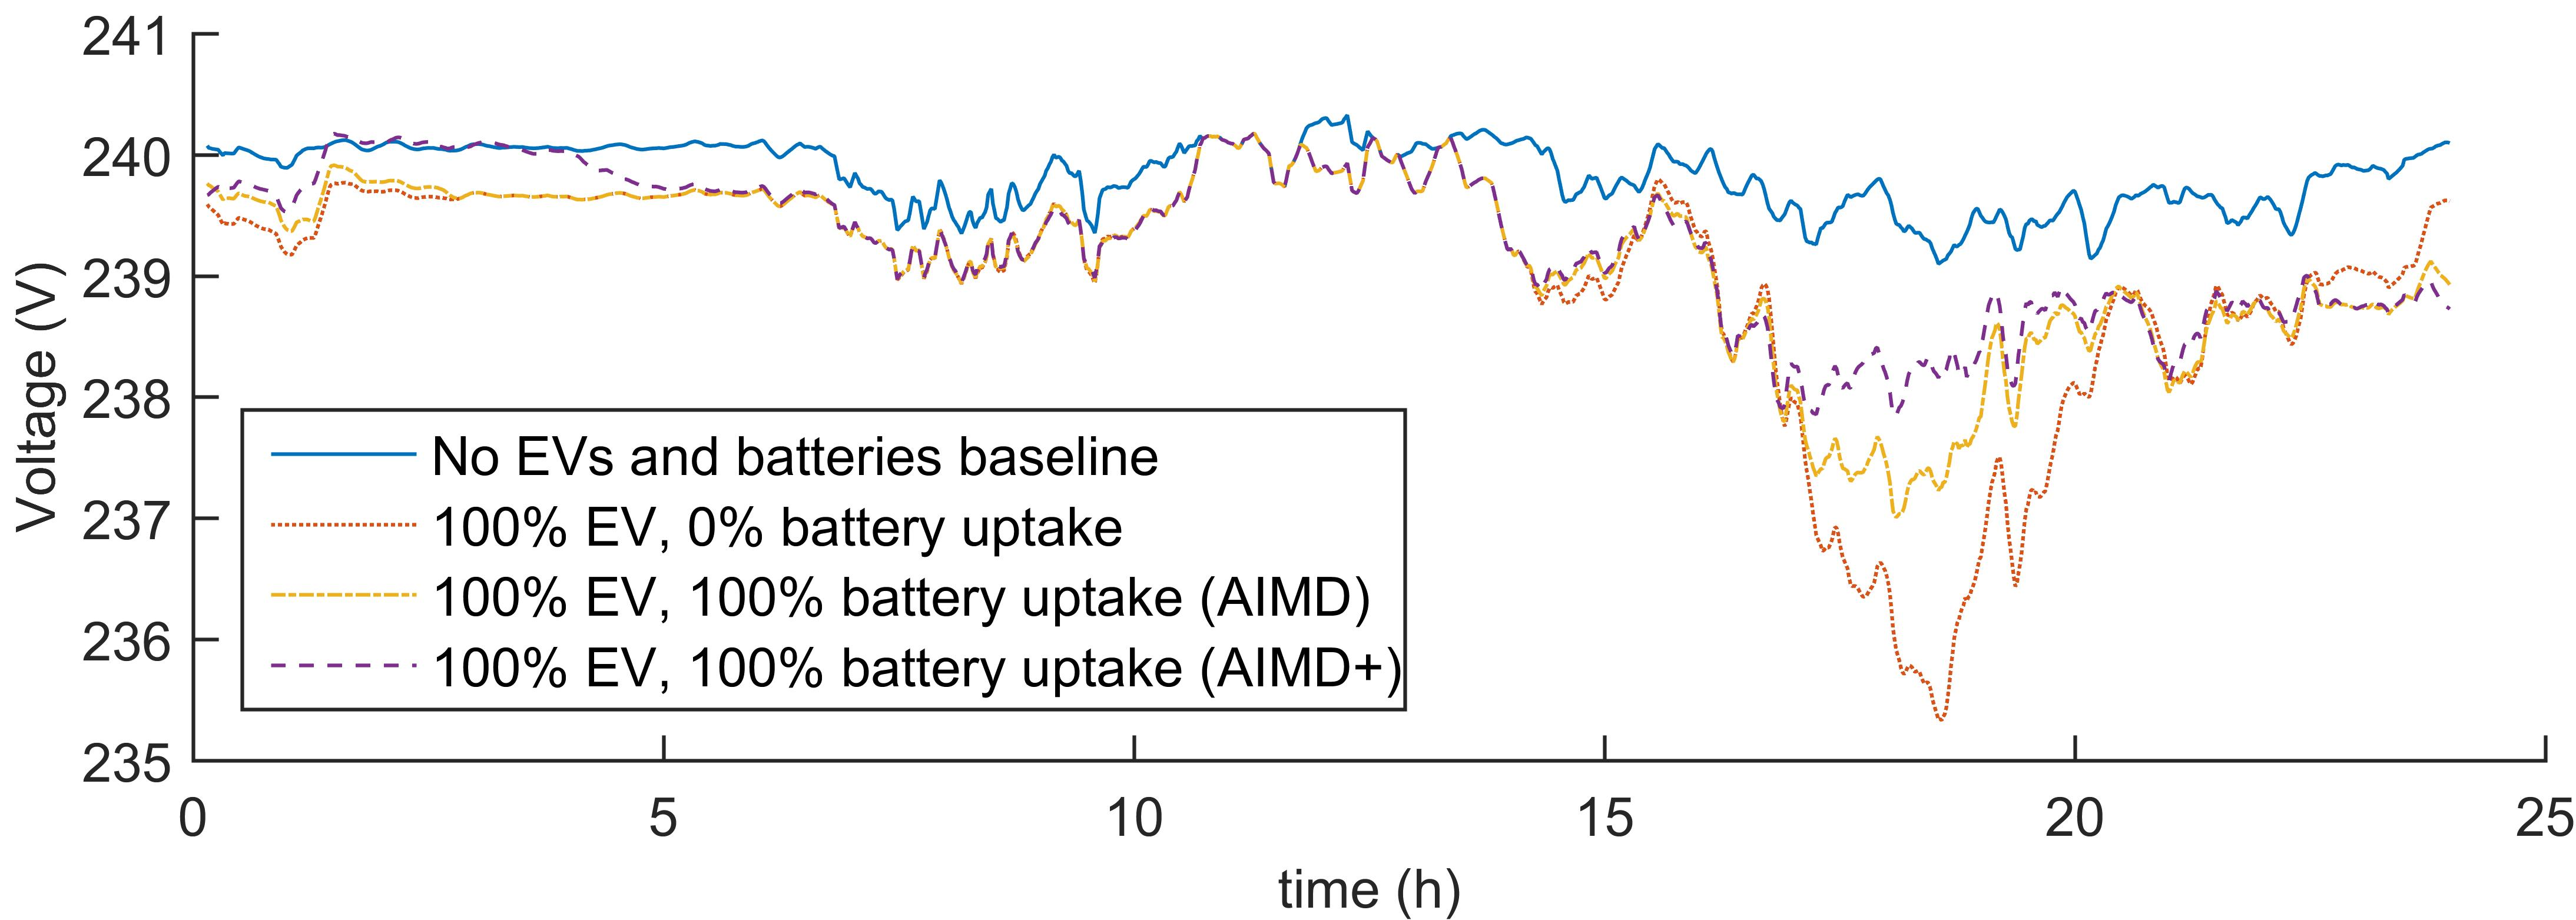
\includegraphics{_chapter1/fig/input/voltage-profiles-excerpt}
	\caption{Recorded voltage profile at the bus of the customer closest to the substation over the period of one day with a certain uptake in EV and battery storage devices using a moving average over a window of 5 min. Here, Case {A} is blue; Case {B} is red; Case {C} is yellow; and Case {D} is violet.}
 \label{ch1:fig:voltage-profiles-excerpt}
\end{figure}


In this histogram, the voltage probability distributions for all four cases were normalised and plotted against each other. Here, the previously seen drop in voltages by introducing EVs is recorded as a shift in the voltage distribution. This voltage drop is mitigated by the introduction of the storage solutions, since the probability distribution is shifted towards higher voltage bands. For the IEEE EU LV Test feeder, the AIMD+-controlled batteries outperform the AIMD devices as the resulting $\zeta_\textbf{C}^{*}$ is greater than $\zeta_\textbf{D}^{*}$.

\begin{figure}[htb]\centering
 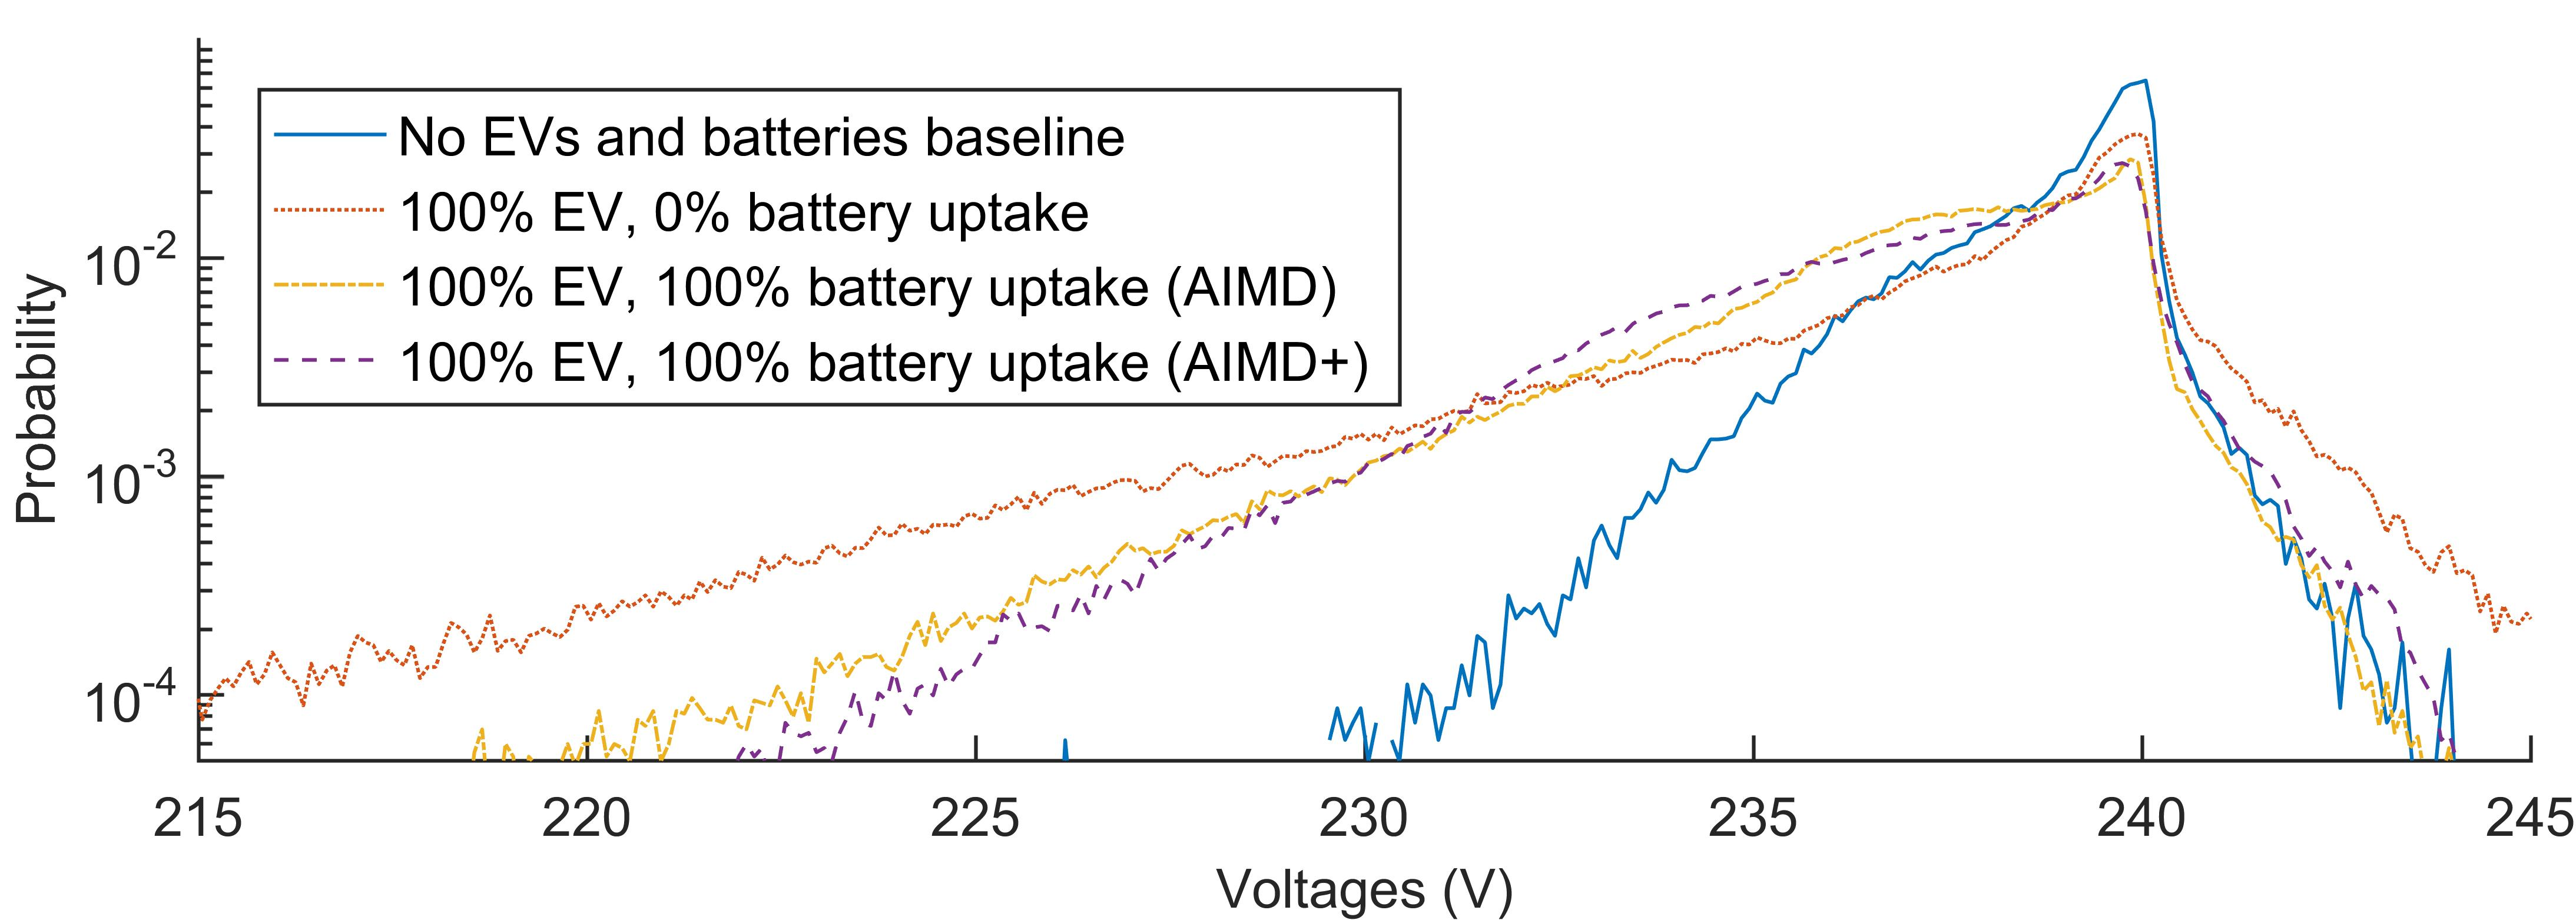
\includegraphics{_chapter1/fig/input/voltage-excerpt}
 \caption{Voltage probability distribution of all loads' buses for certain uptakes of EV and battery storage devices. Here, Case {A} is blue; Case {B} is red; Case {C} is yellow; and Case {D} is violet; with $\zeta_\textbf{C}^{*} = -0.153$ and $\zeta_\textbf{D}^{*}=-0.135$.}
 \label{ch1:fig:voltage-violation-excerpt}
\end{figure}


To gain a full understanding of the performance of the AIMD and AIMD+ algorithms, a full sweep of EV and BESS uptake combinations was simulated on all available power distribution networks. The resulting parameters were averaged and plotted in Figure \ref{ch1:fig:voltage-comparison-large}.

\begin{figure}[htb]\centering
\subfloat[]{%
	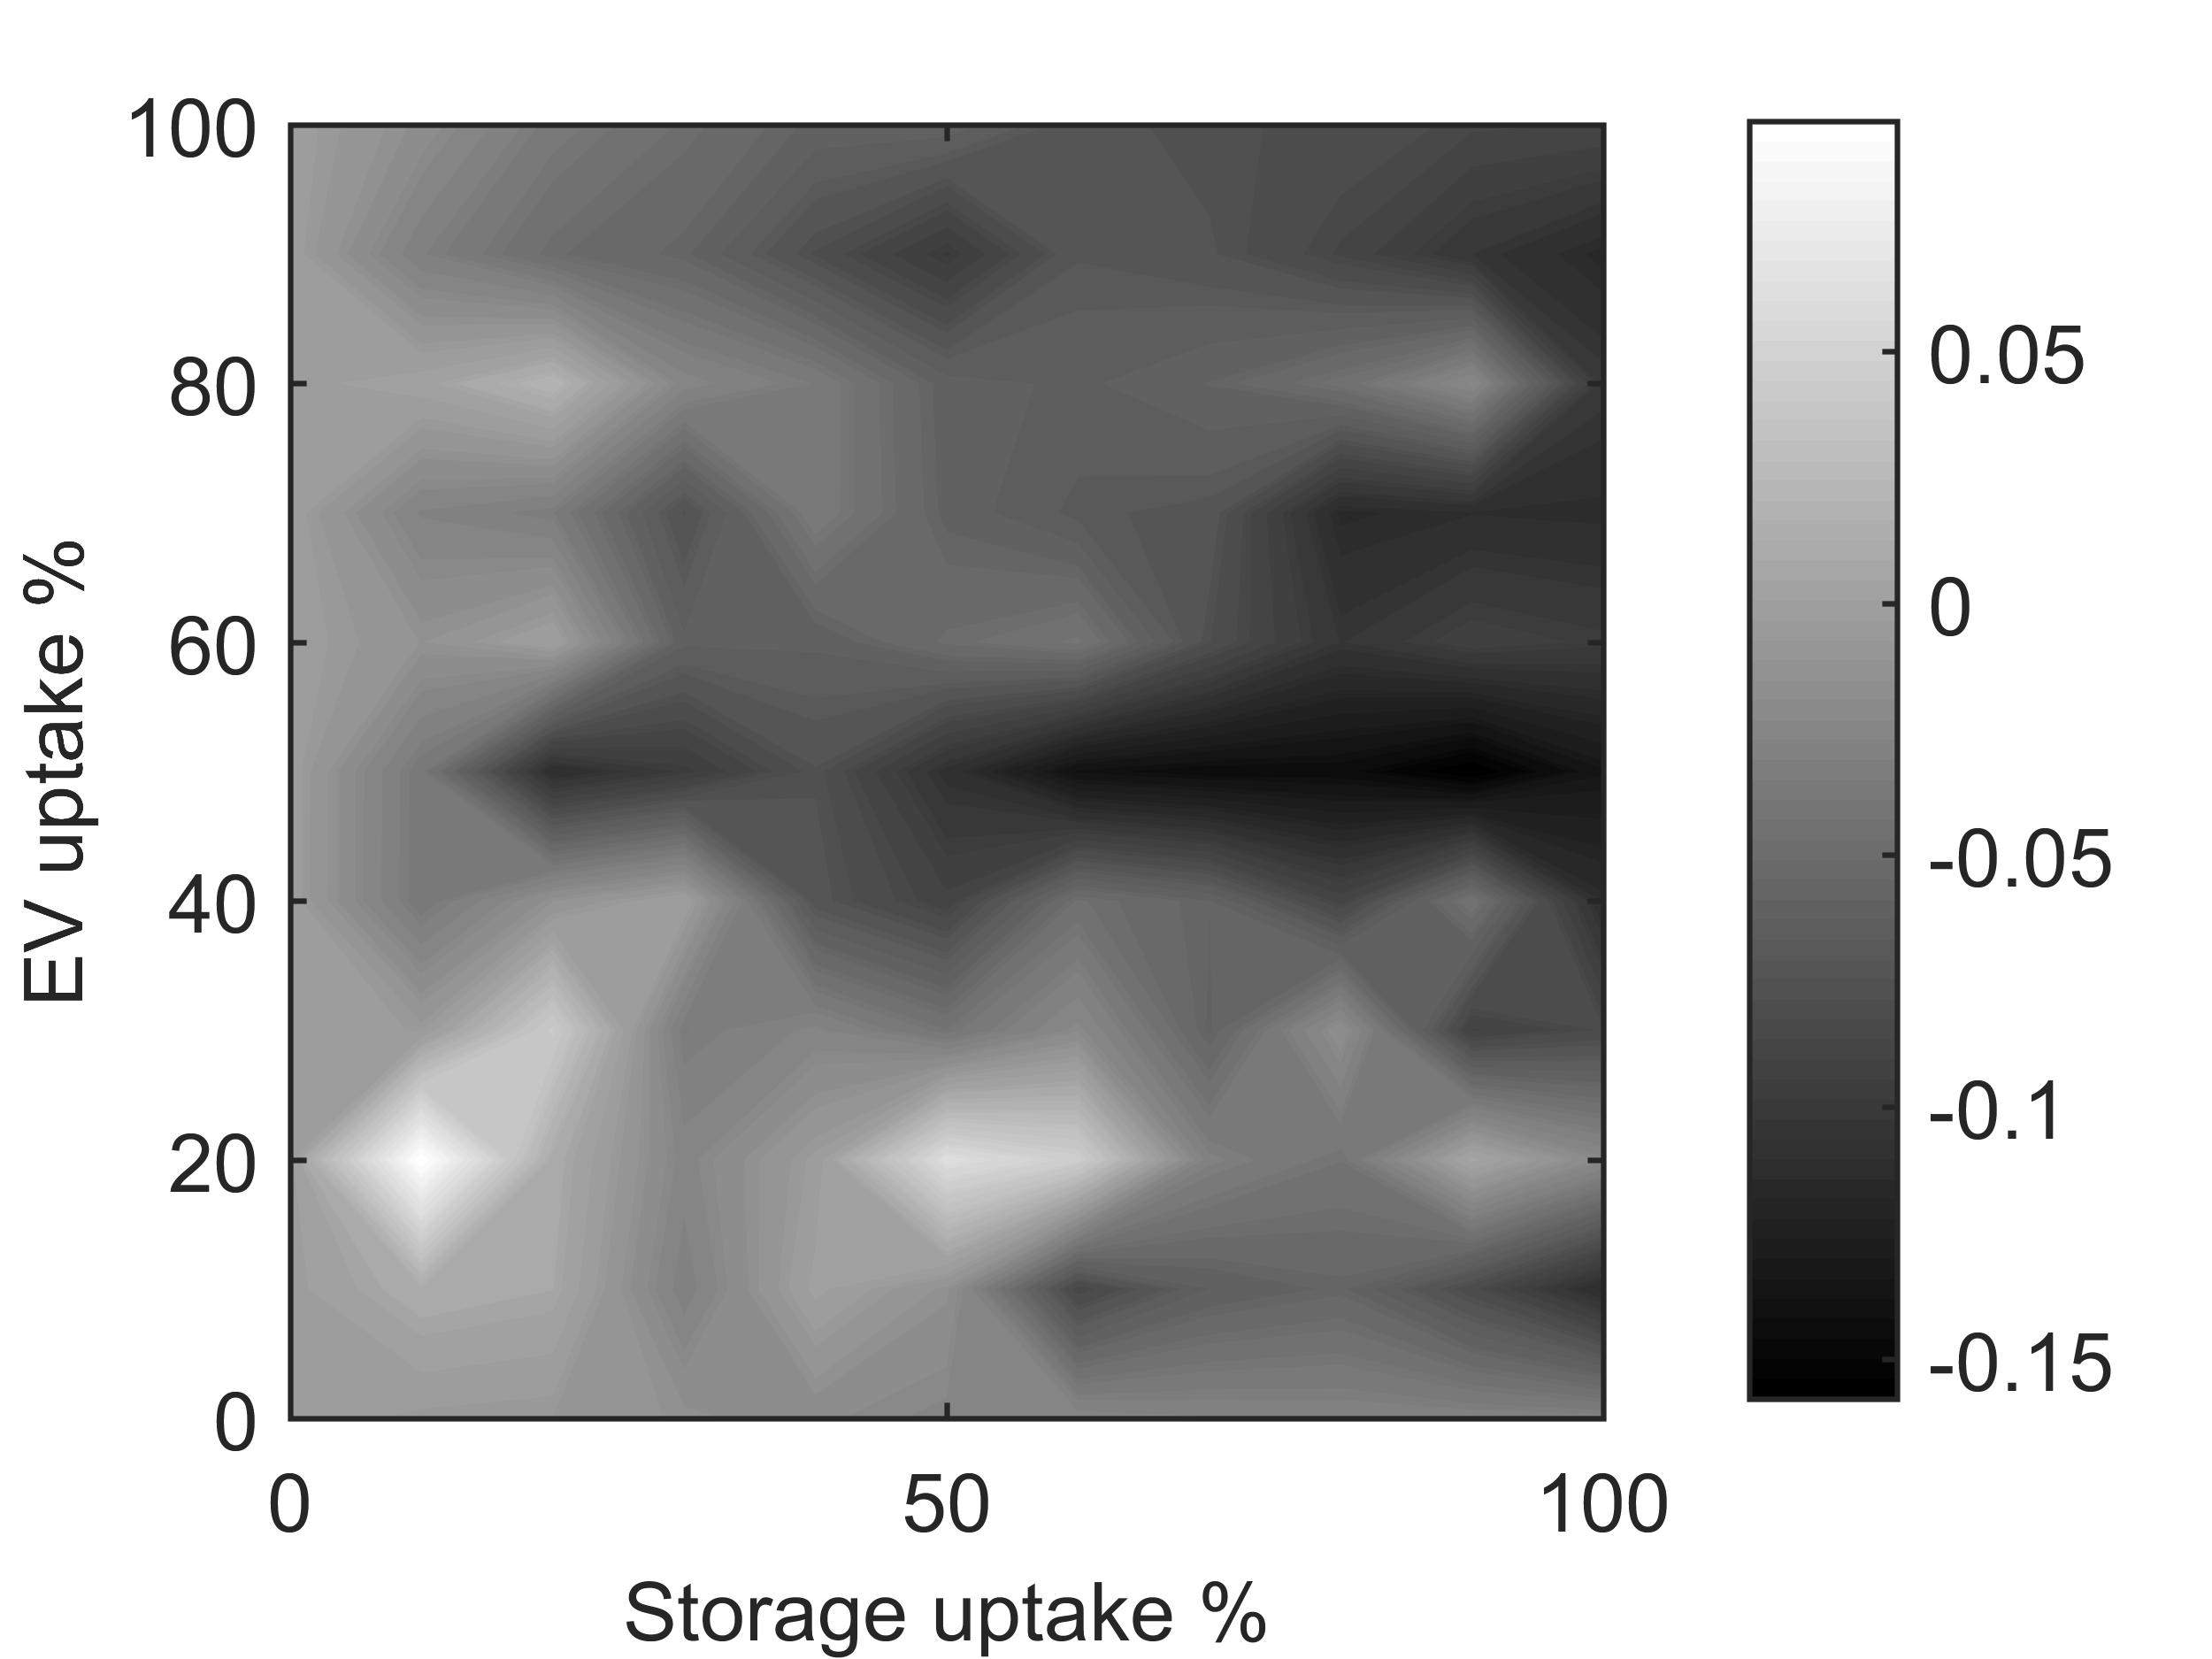
\includegraphics[width=0.48\textwidth]{_chapter1/fig/input/voltage-AIMD1}%
 	\label{ch1:subfig:voltage-AIMD1}%
}
\subfloat[]{%
	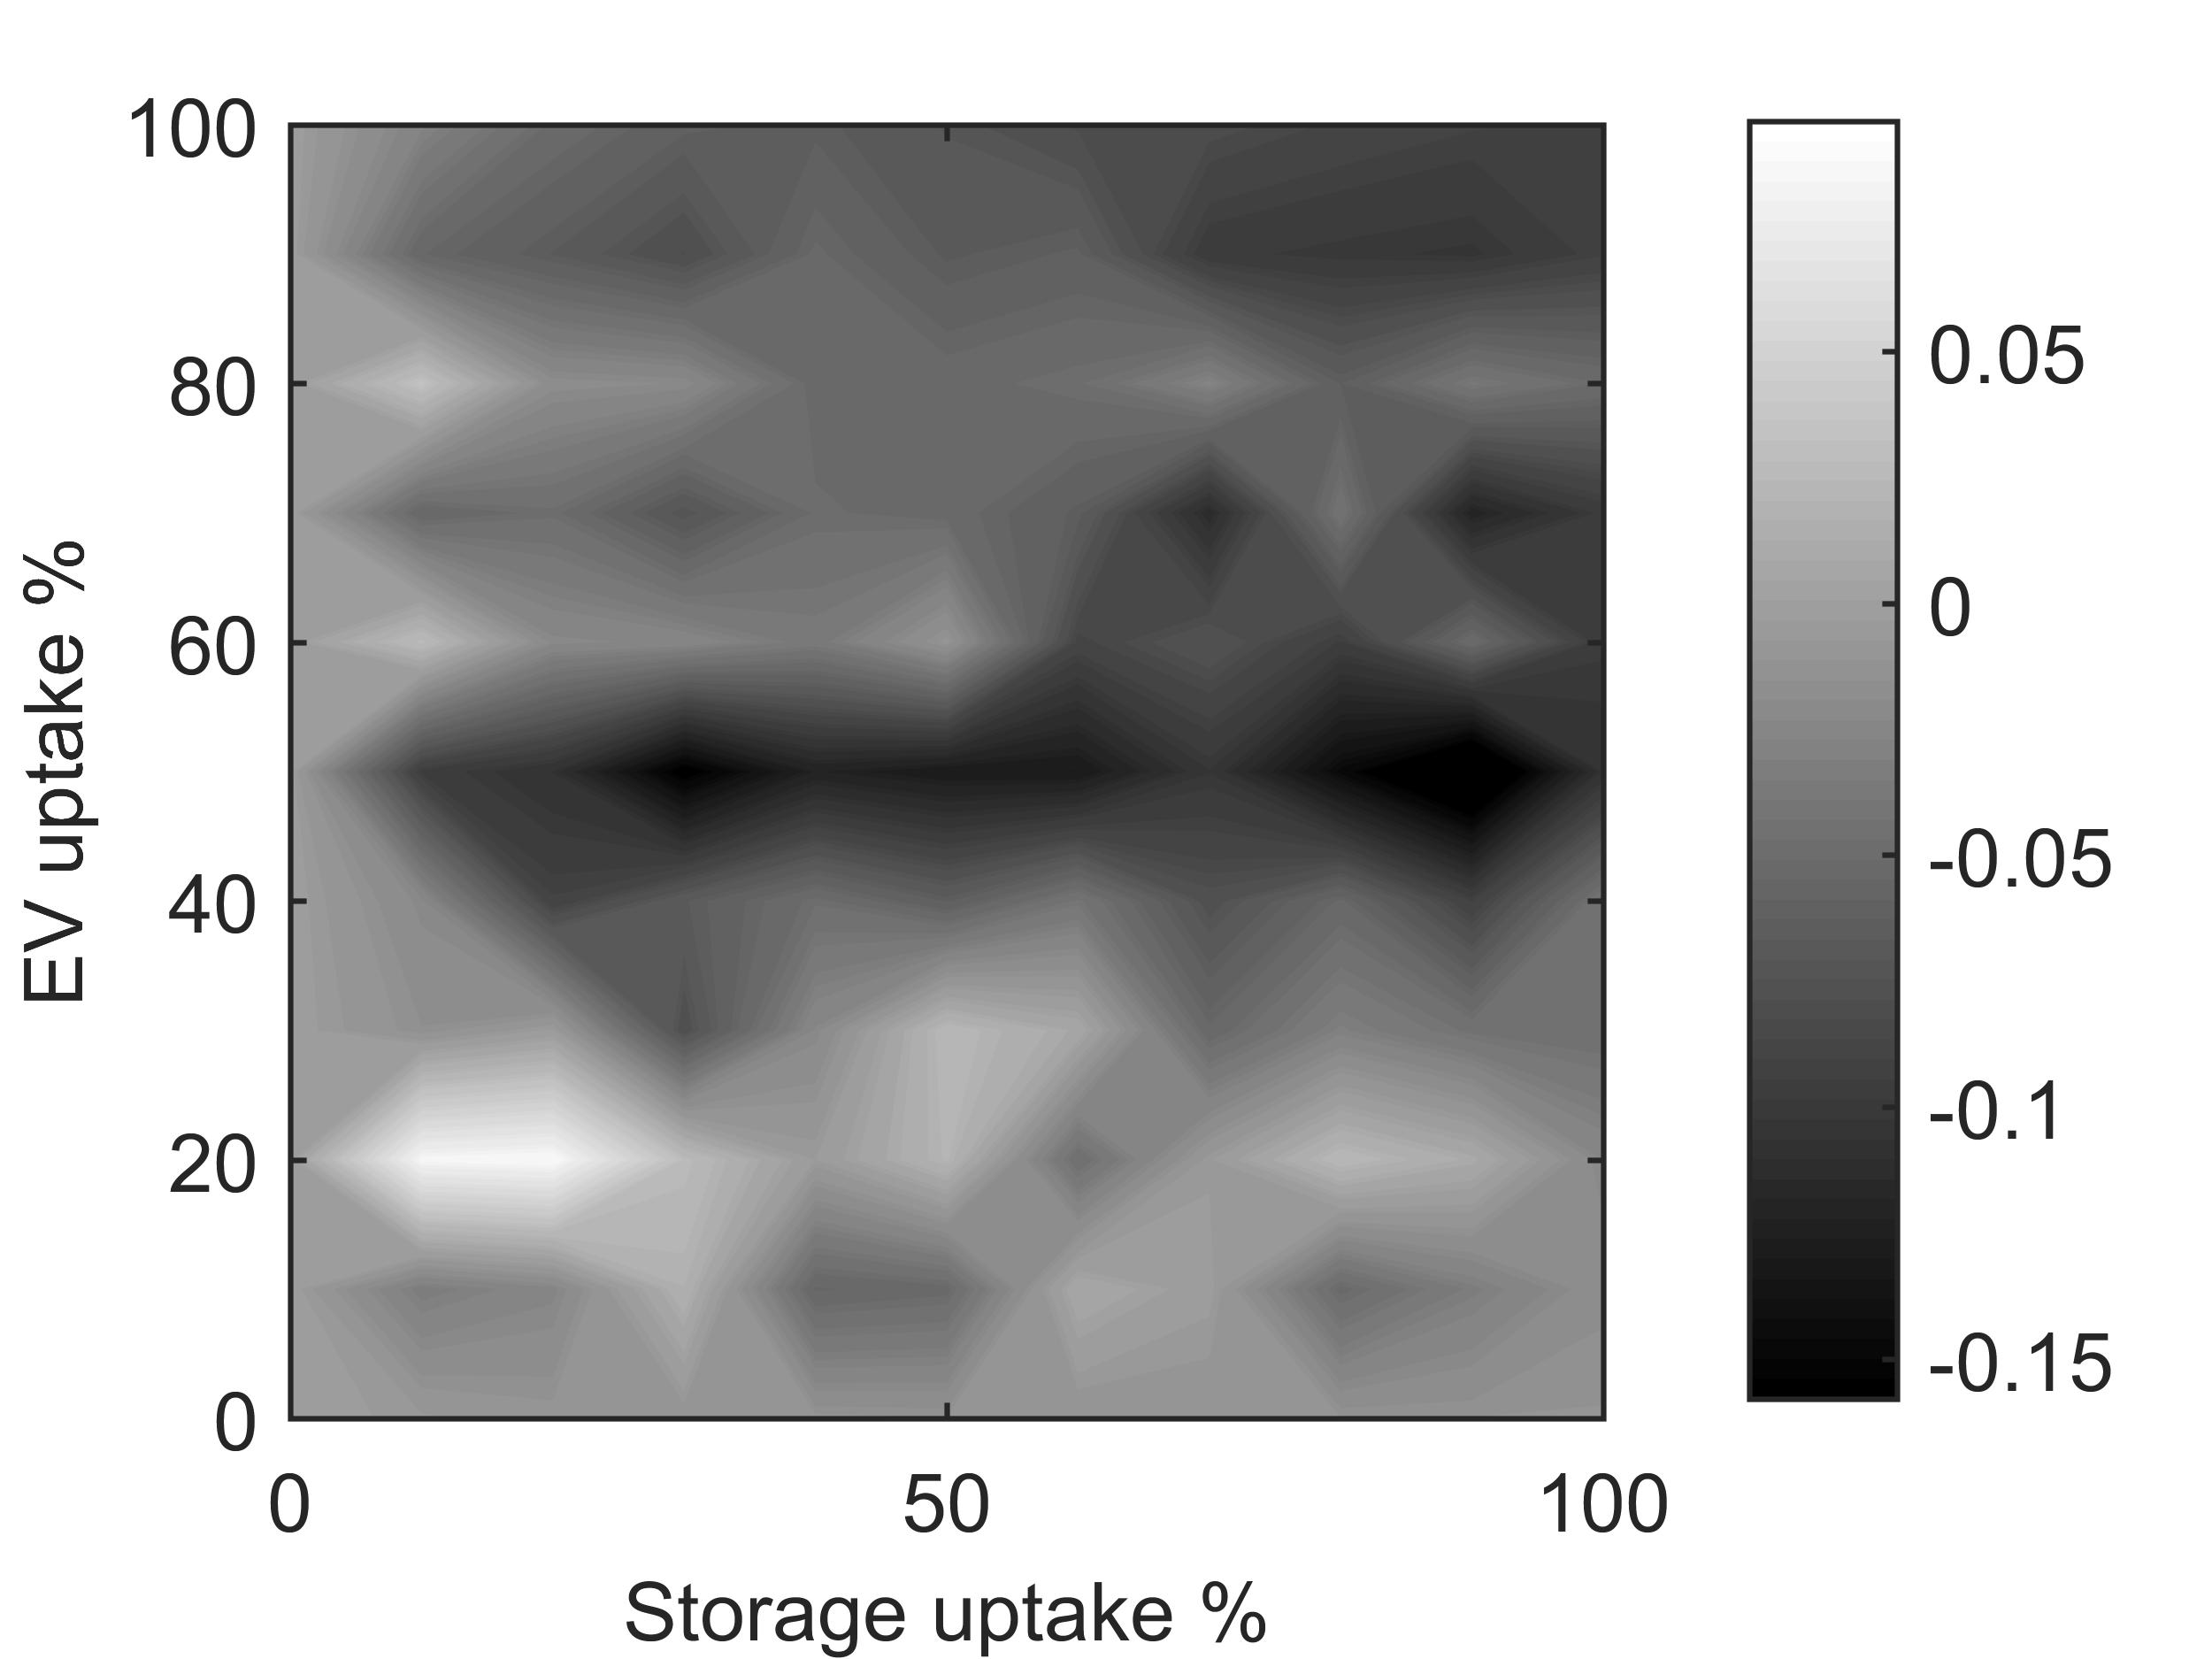
\includegraphics[width=0.48\textwidth]{_chapter1/fig/input/voltage-AIMD2}%
	\label{ch1:subfig:voltage-AIMD2}%
}
\caption{Comparison of voltage improvement indices (i.e., $\zeta^{*}$) for (\textbf{a}) AIMD, i.e. $\zeta_\textbf{C}^{*}$, and (\textbf{b}) AIMD+, i.e. $\zeta_\textbf{D}^{*}$.}
 \label{ch1:fig:voltage-comparison-large}
\end{figure}


These figures show that the AIMD+ control algorithm reduces voltage deviation more effectively as the uptake in storage and EVs increases. For low storage uptake, the AIMD algorithm does not perform as strongly since more $\zeta_\textbf{C}^{*}$ values are positive and larger than their corresponding $\zeta_\textbf{D}^{*}$ value. This becomes more apparent when averaging all $\zeta_\textbf{C}^{*}$ and $\zeta_\textbf{D}^{*}$ values for their common storage uptake and across all EV uptakes. The resulting averaged metrics are plotted in Figure \ref{ch1:fig:voltage-aimd-compare}.

In this last figure, it can be seen how the sole impact of BESS uptake reflects in a continuing improvement of voltage levels. In fact, both compared algorithms improved the bus voltage, which coincides with the findings in the case studies. On average, this is the case for all BESS uptakes, as $\zeta_\textbf{C}^{*} \approx \zeta_\textbf{D}^{*}$. Nonetheless, it should be noted that the AIMD+ algorithm had reduced the frequency of severe voltage deviations in comparison to the AIMD algorithm and is more effective during scenarios with lower BESS uptake.

\begin{figure}[htb]\centering
 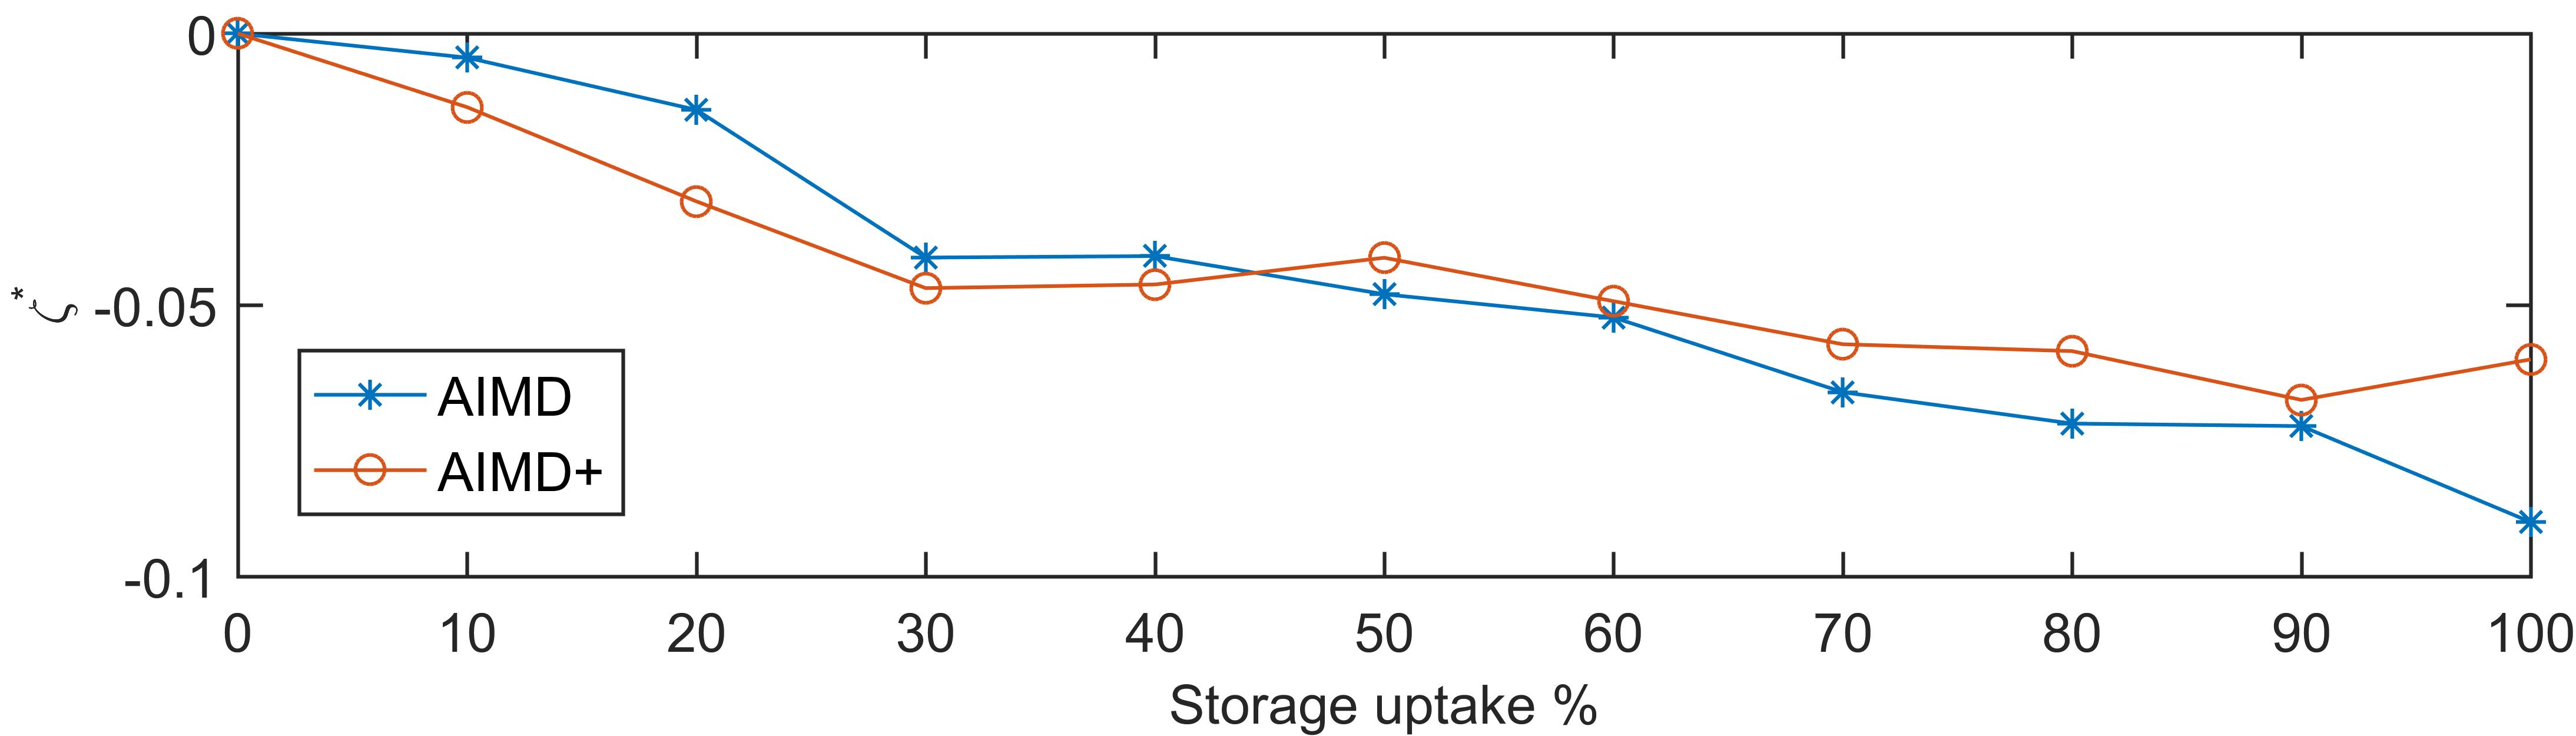
\includegraphics{_chapter1/fig/input/voltage-AIMD-compare}
 \caption{Average $\zeta_\textbf{C}^{*}$ (AIMD) and $\zeta_\textbf{D}^{*}$ (AIMD+) values recorded against the corresponding storage~uptake.}
 \label{ch1:fig:voltage-aimd-compare}
\end{figure}


\subsection{Line Overload Analysis}

Similar to the voltage improvement analysis, a frequency distribution of the line utilisation was generated. Figure \ref{ch1:fig:line-utilisation-excerpt} shows a probability distribution of the per unit (1 p.u. represents a 100\% line usage, i.e., a line current of the same value as the line's nominal current rating) current in all lines, for each of the four scenarios. The corresponding $\zeta_\textbf{C}^{**}$ and $\zeta_\textbf{D}^{**}$ values for the AIMD and AIMD+ storage deployment have also been included in the figure's caption. In this figure, the observed high probability of line over-utilisation confirms that the used test network is of insufficient capacity to cater for the chosen EV uptake.

\begin{figure}[htb]\centering
 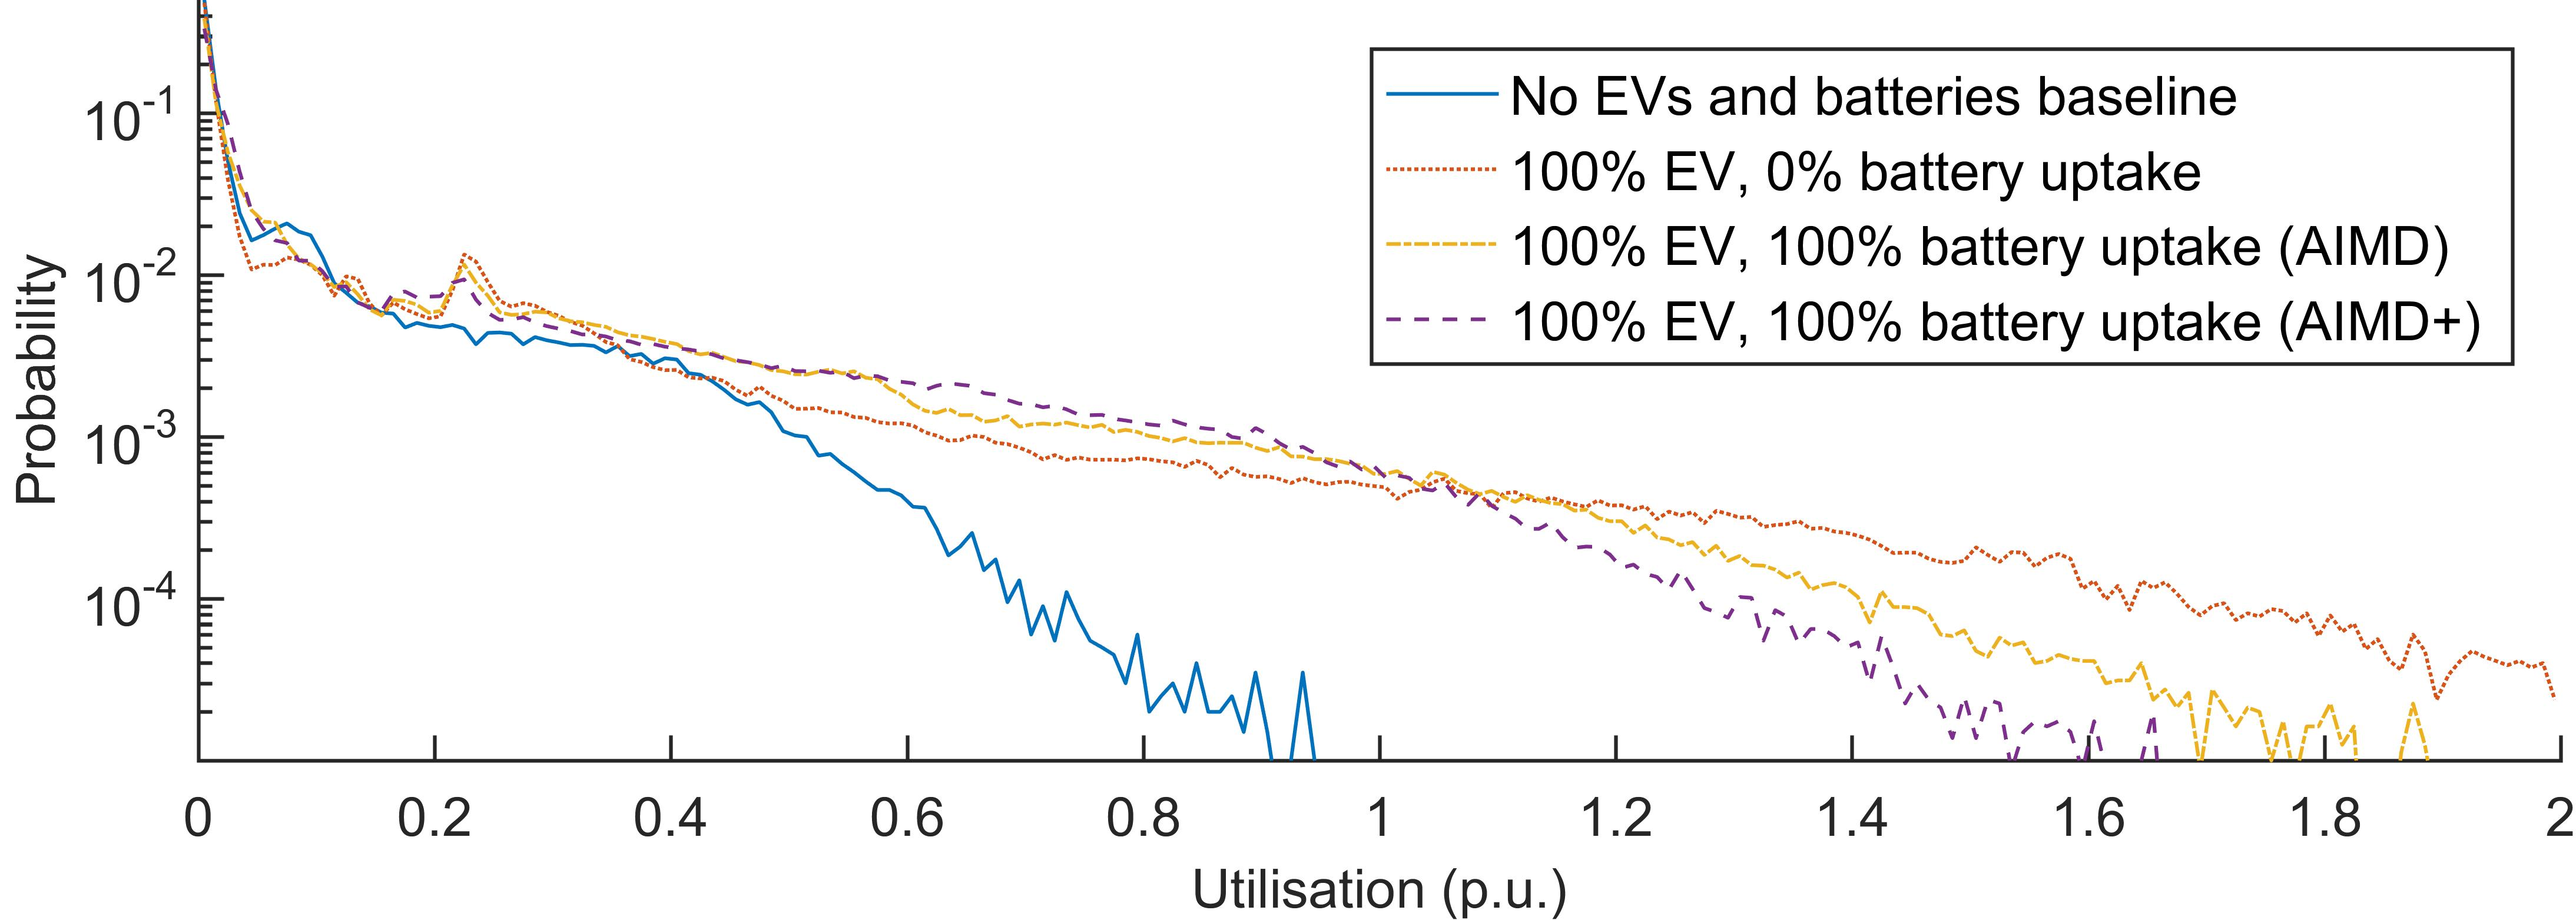
\includegraphics{_chapter1/fig/input/utilisation-excerpt}
 \caption{Line utilisation probability distribution of all lines in the simulated feeder for certain uptakes of EV and battery storage devices. Here, Case {A} is blue; Case {B} is red; Case {C} is yellow; and Case {D} is violet; with $\zeta_\textbf{C}^{**} = -0.360$ and $\zeta_\textbf{D}^{**} = -0.518$.}
 \label{ch1:fig:line-utilisation-excerpt}
\end{figure}


Here, the AIMD+ controlled storage devices yielded a noticeable reduction in line overloads. This improvement is apparent through the compressed width of the probability distribution and the negative $\zeta_\textbf{D}^{**}$ value. In contrast, the AIMD controlled storage devices do not fully utilise the line capacity as effectively, which leads to a positive value of $\zeta_\textbf{C}^{**}$. To evaluate the line utilisation improvement across all simulations, the full range of EV and storage uptake was evaluated. The resulting plots are shown in Figure \ref{ch1:fig:utilisation-comparison-large}.

In these figures, it can be seen how the performance metrics change as EV uptake and storage uptake increase. For the AIMD-controlled BESS, the resulting $\zeta_\textbf{C}^{**}$ values are distributed around zero, whereas the AIMD+ algorithm achieved mostly negative values of $\zeta_\textbf{D}^{**}$. These negative values confirm the better usage of available line capacity. This becomes particularly noticeable for scenarios where very low EV uptake is combined with larger BESS uptake. Here, AIMD-controlled storage devices commence their initial charge simultaneously. As they are located closer to the substation, they do not measure a sufficient bus voltage offset to regulate down their charging power. This behaviour causes a number of line overloads at the very beginning of the simulated days. The AIMD+ algorithm on the other hand, with its adjusted thresholds, is more responsive to non-optimal network operation and, therefore, increases the charging rate gradually.

\begin{figure}[htb]\centering
\subfloat[]{%
	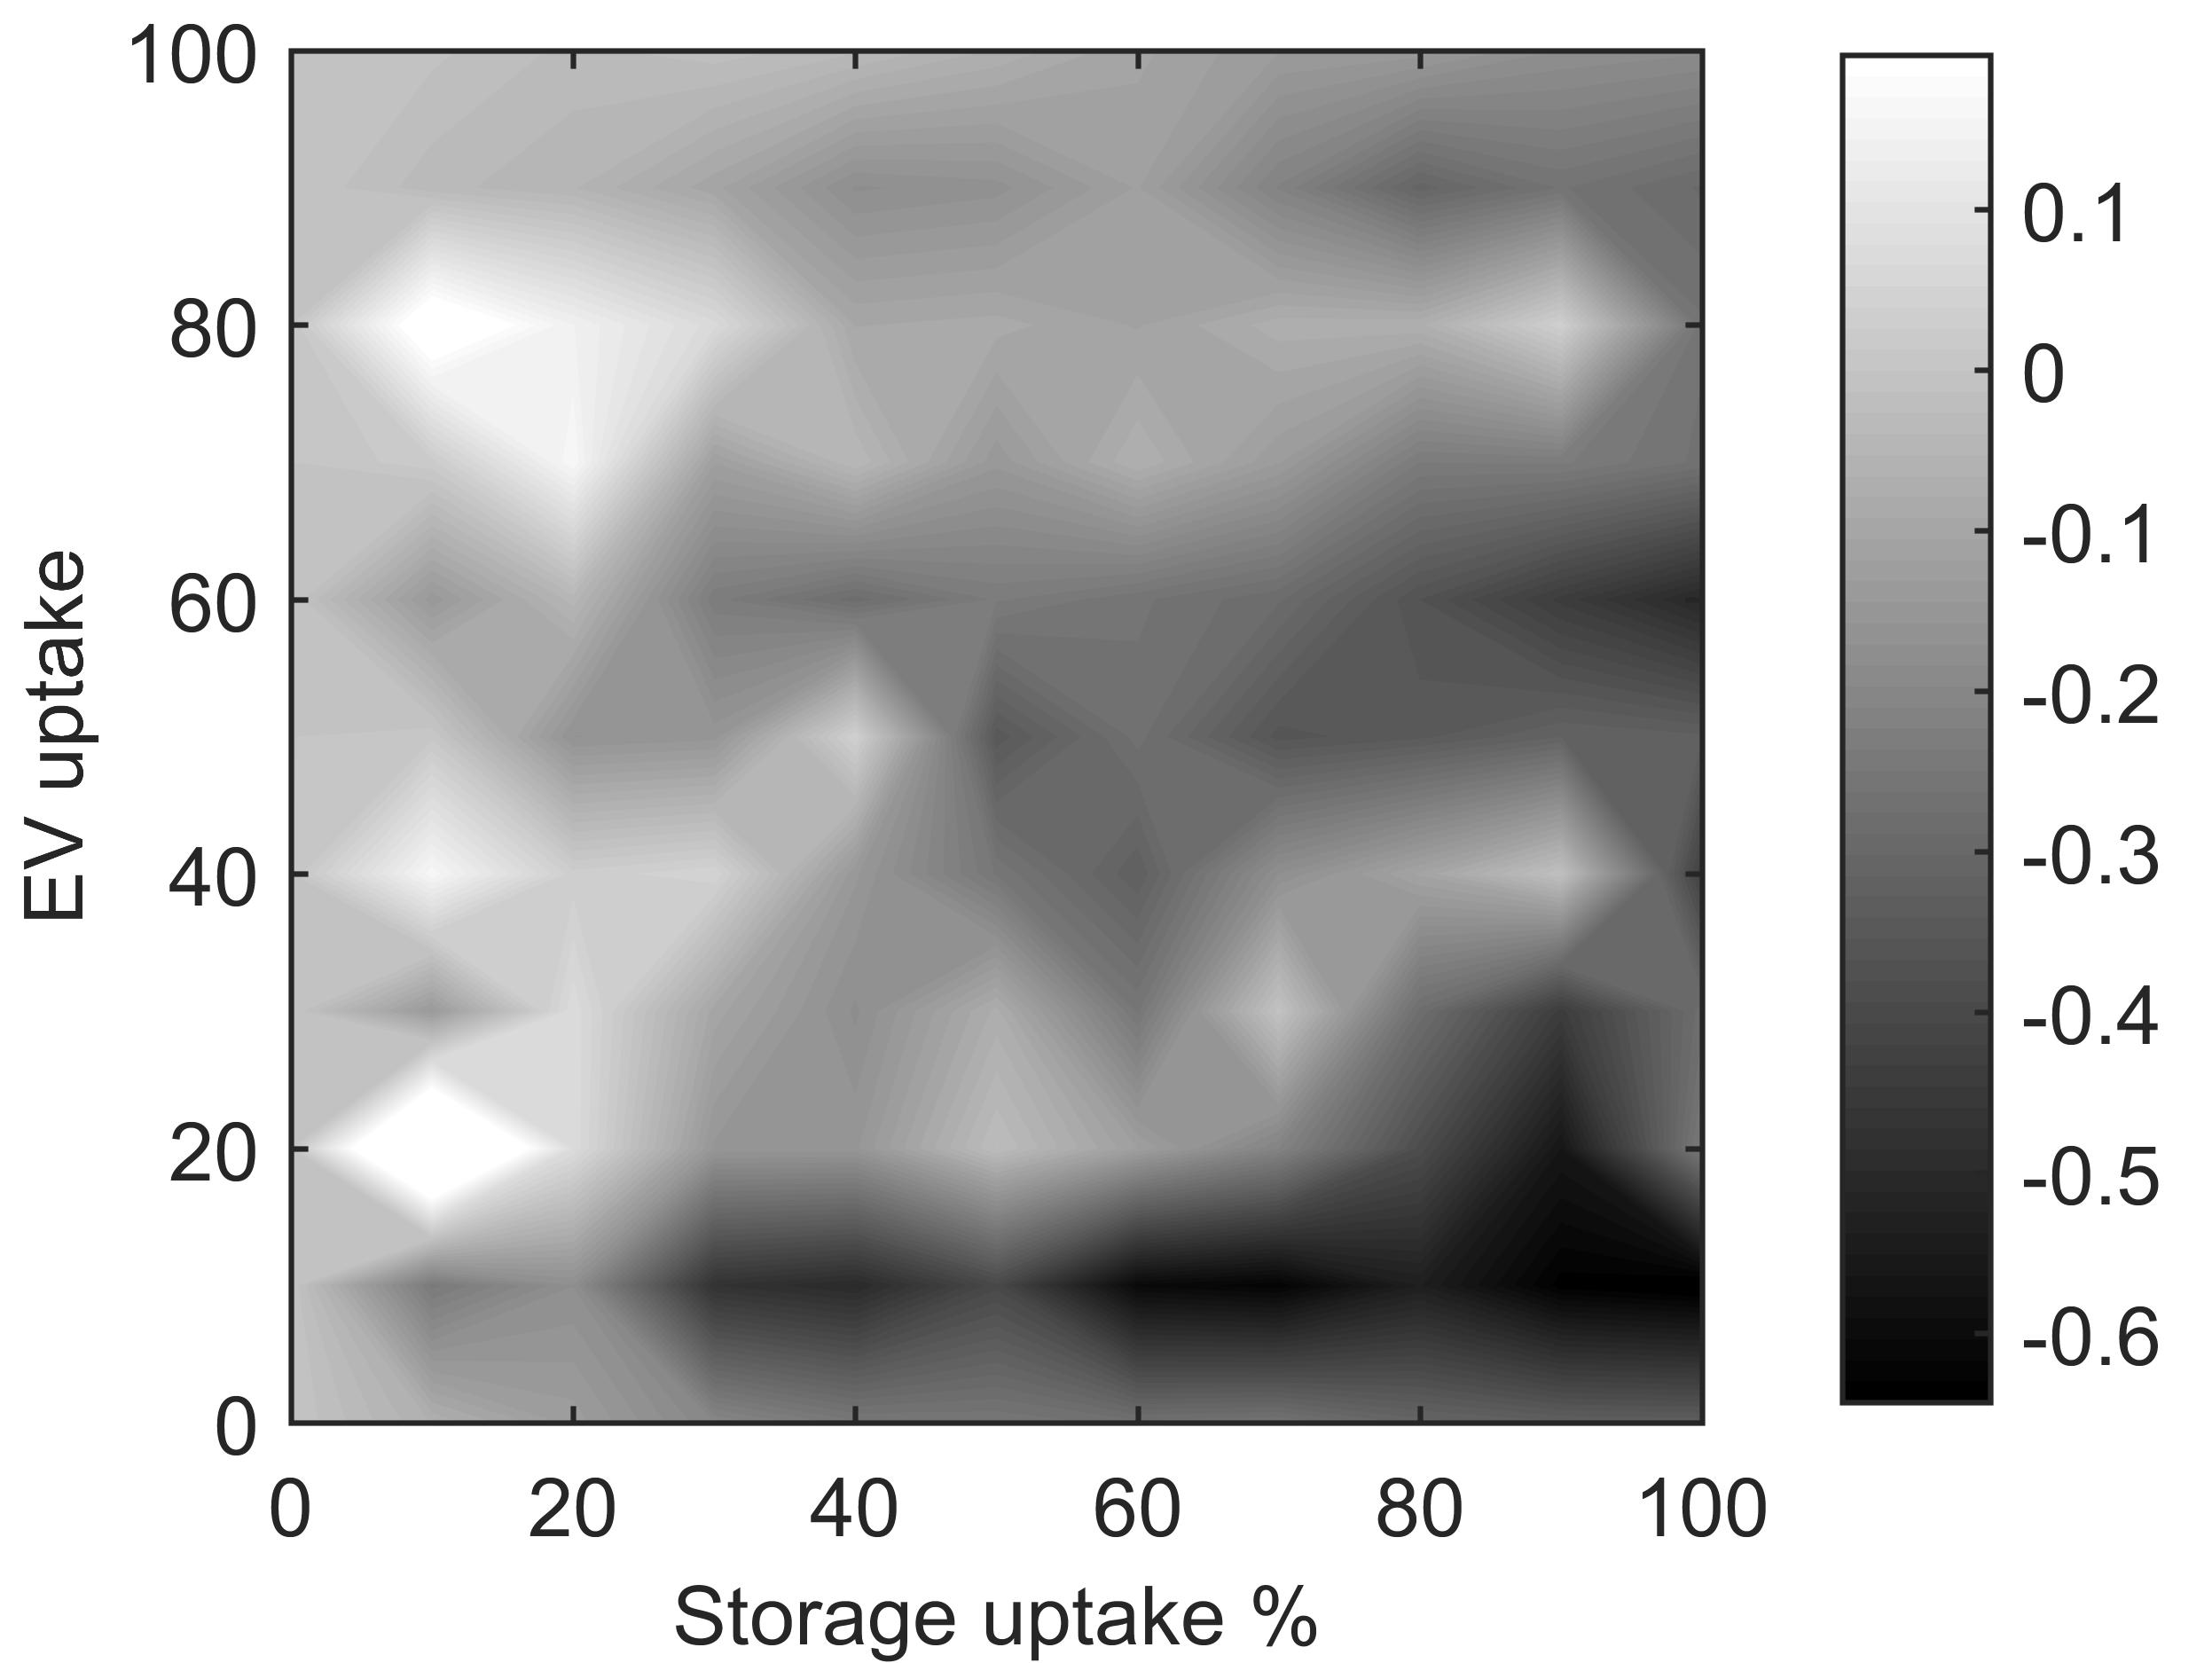
\includegraphics[width=0.48\textwidth]{_chapter1/fig/input/utilisation-AIMD1}%
	\label{subfig-utilisation-AIMD1}%
}
\subfloat[]{%
	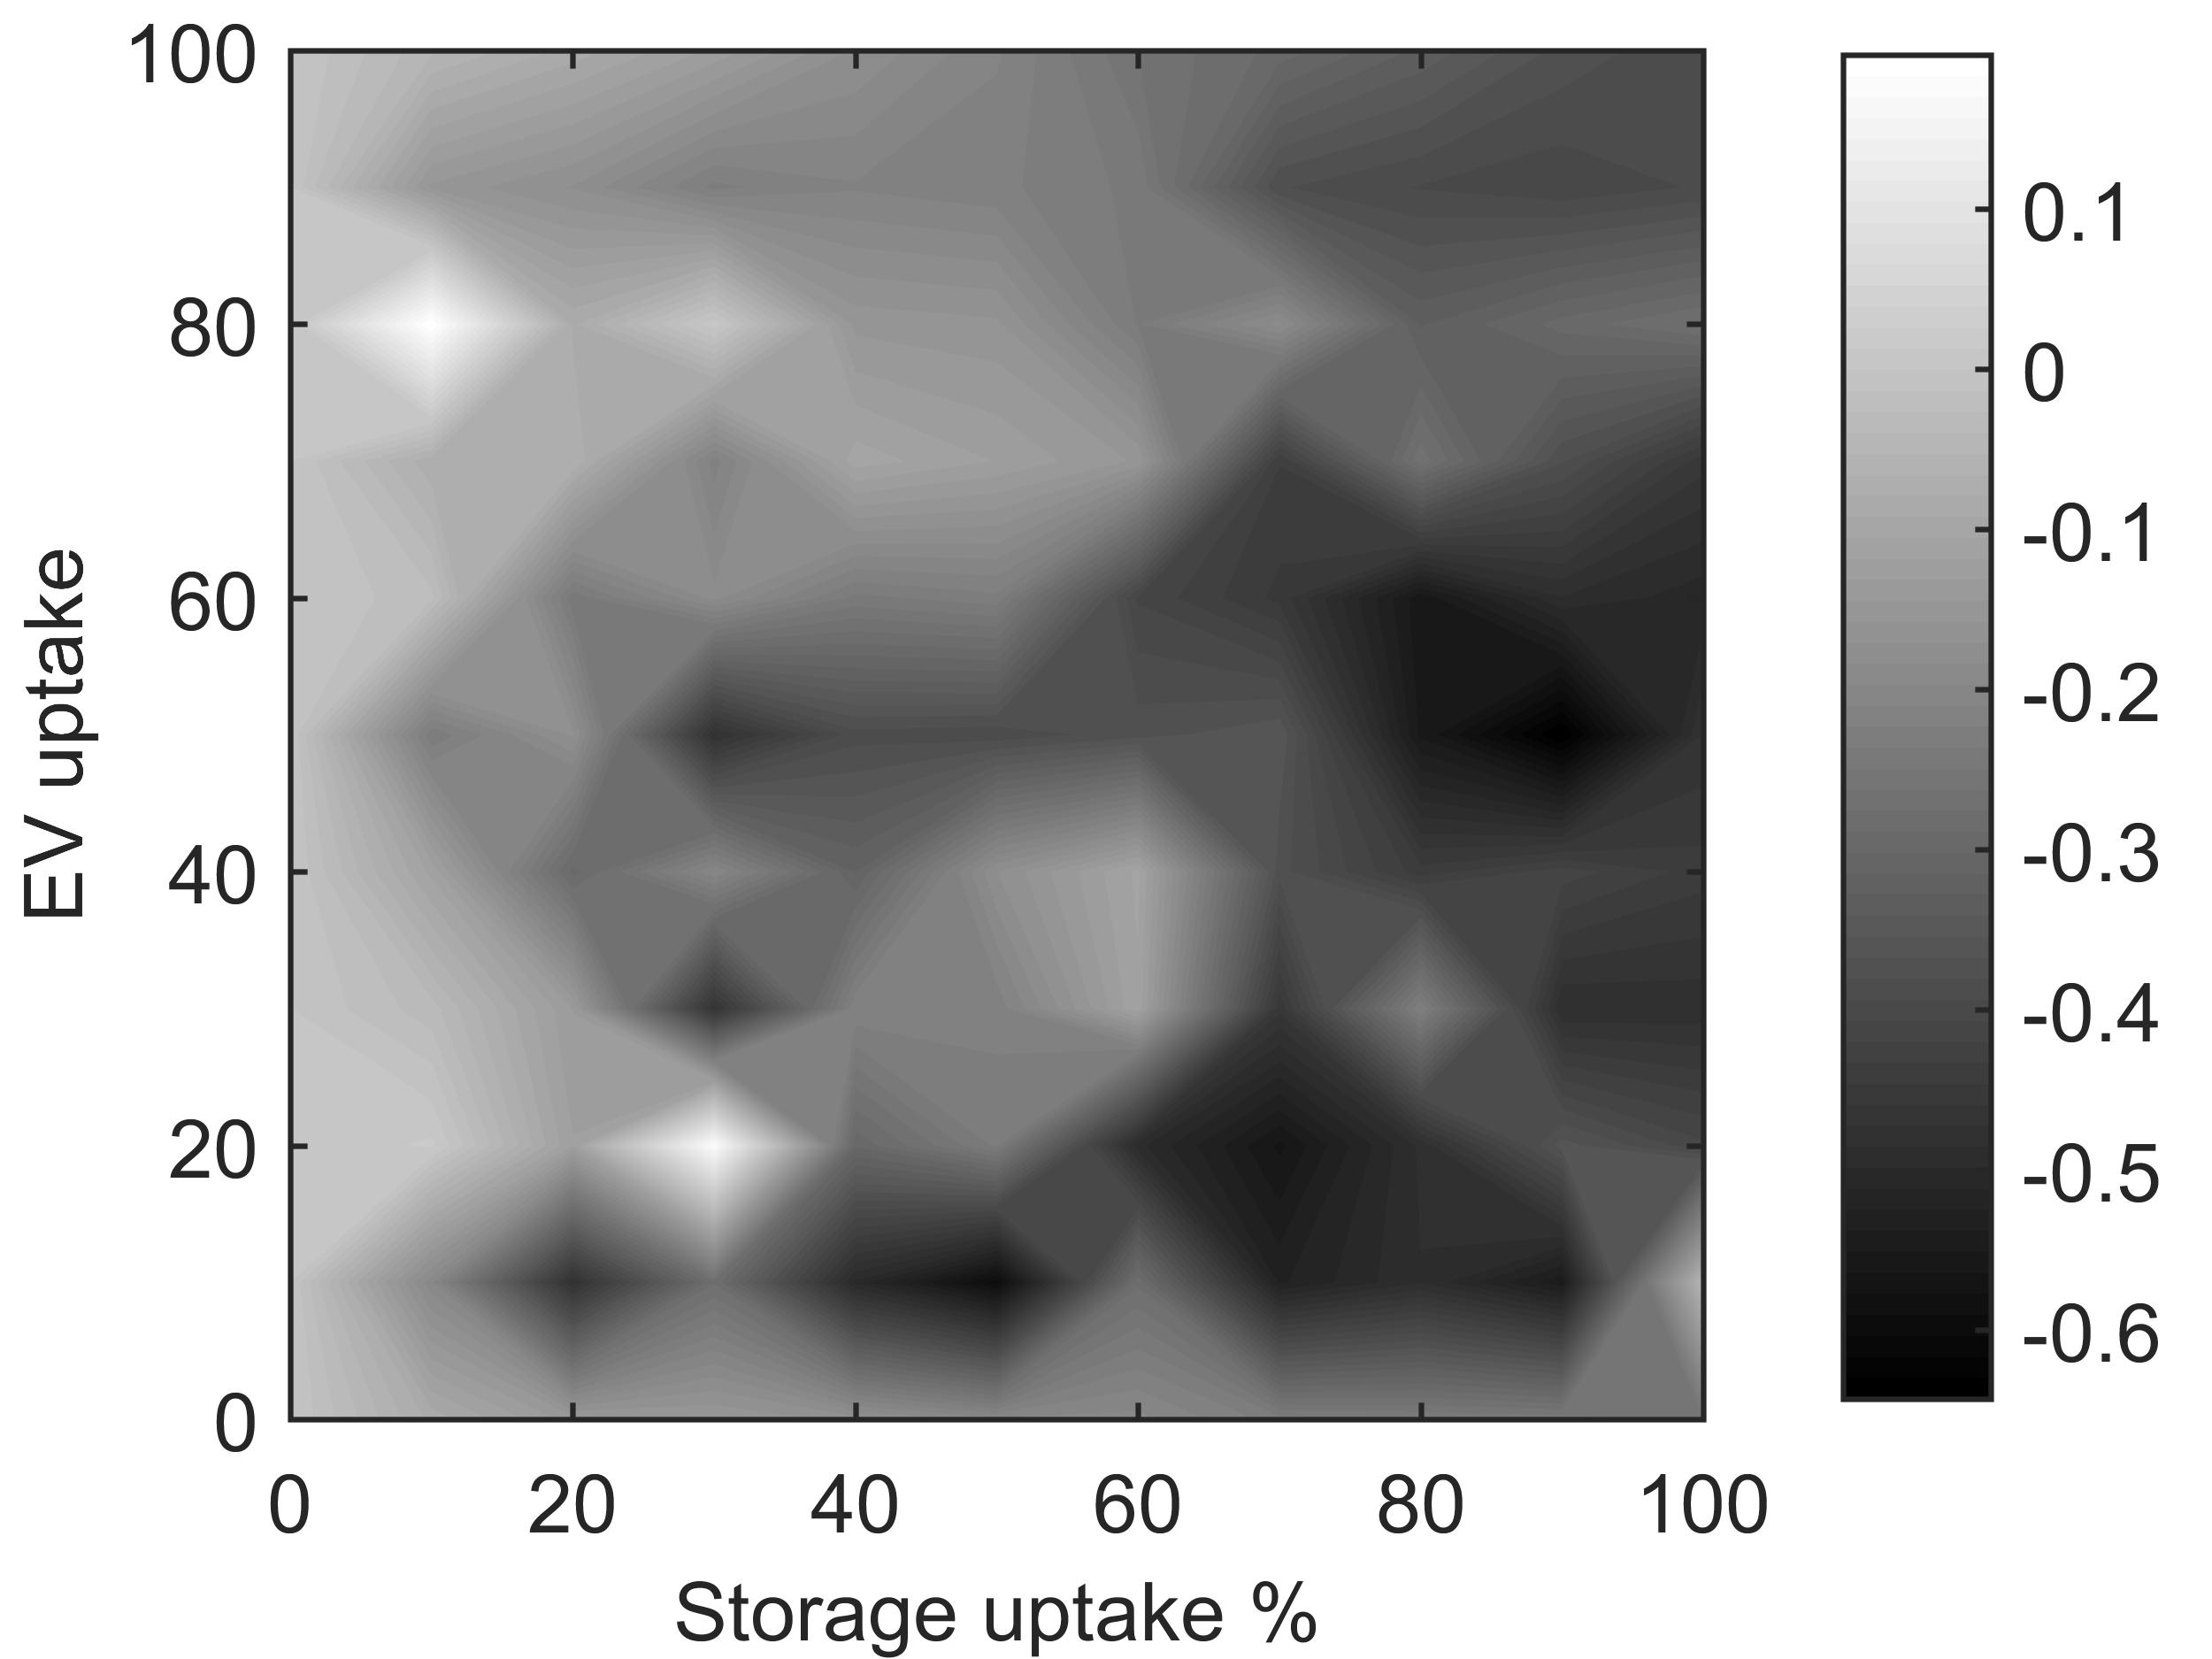
\includegraphics[width=0.48\textwidth]{_chapter1/fig/input/utilisation-AIMD2}%
	\label{subfig-utilisation-AIMD2}%
}
\caption{Comparison of line utilisation improvement indices for (\textbf{a}) AIMD and (\textbf{b}) AIMD+. ({a})~$\zeta_\textbf{C}^{**}$~indices (AIMD); ({b}) $\zeta_\textbf{D}^{**}$ indices (AIMD+).}
\label{ch1:fig:utilisation-comparison-large}
\end{figure}


This gradual adjustment is based on the fact that the bus voltages in the AIMD+ algorithm are closer to their nominal voltages (i.e., bus voltages found by simulating the feeder with its equally-distributed nominal load) than they are in the conventional AIMD case. A greater voltage disparity, which is the case in AIMD, causes a prolonged additive adjustment to the battery's power. This prolonged adjustment is particularly apparent for batteries situated at the bottom of the feeder, as their voltage measurements deviate the furthest from the substation voltage level. AIMD+ on the other hand prevents this behaviour by setting the voltage threshold based on the network's nominal voltage drop, which is dependent on the distance between the BESS and its feeding substation. As a result, the set-point voltage thresholds at the bottom of the feeder are lower than those closer to the substation. Hence, the additive power adjustment is equalised along the entire feeder. Therefore, by applying these individualised control thresholds, the sensitivity of the algorithm is corrected, whilst successfully mitigating the severity of line overloads.

Averaging the $\zeta_\textbf{C}^{**}$ and $\zeta_\textbf{D}^{**}$ values over all EV uptakes gives a clearer indication of performance, as this is now the only variable in the performance analysis. The result is plotted in Figure \ref{ch1:fig:utilisation-aimd-compare}. Here, the hypothesis that AIMD-controlled energy storage devices do not improve line utilisation is confirmed. In contrast, the AIMD+-controlled devices succeed at effectively reducing line overloads. This is also demonstrated by the values of $\zeta_\textbf{C}^{**}$, which remain positive yet close to zero, whereas $\zeta_\textbf{D}^{**}$ decreases with increasing uptake of battery storage devices.

\begin{figure}[htb]\centering
 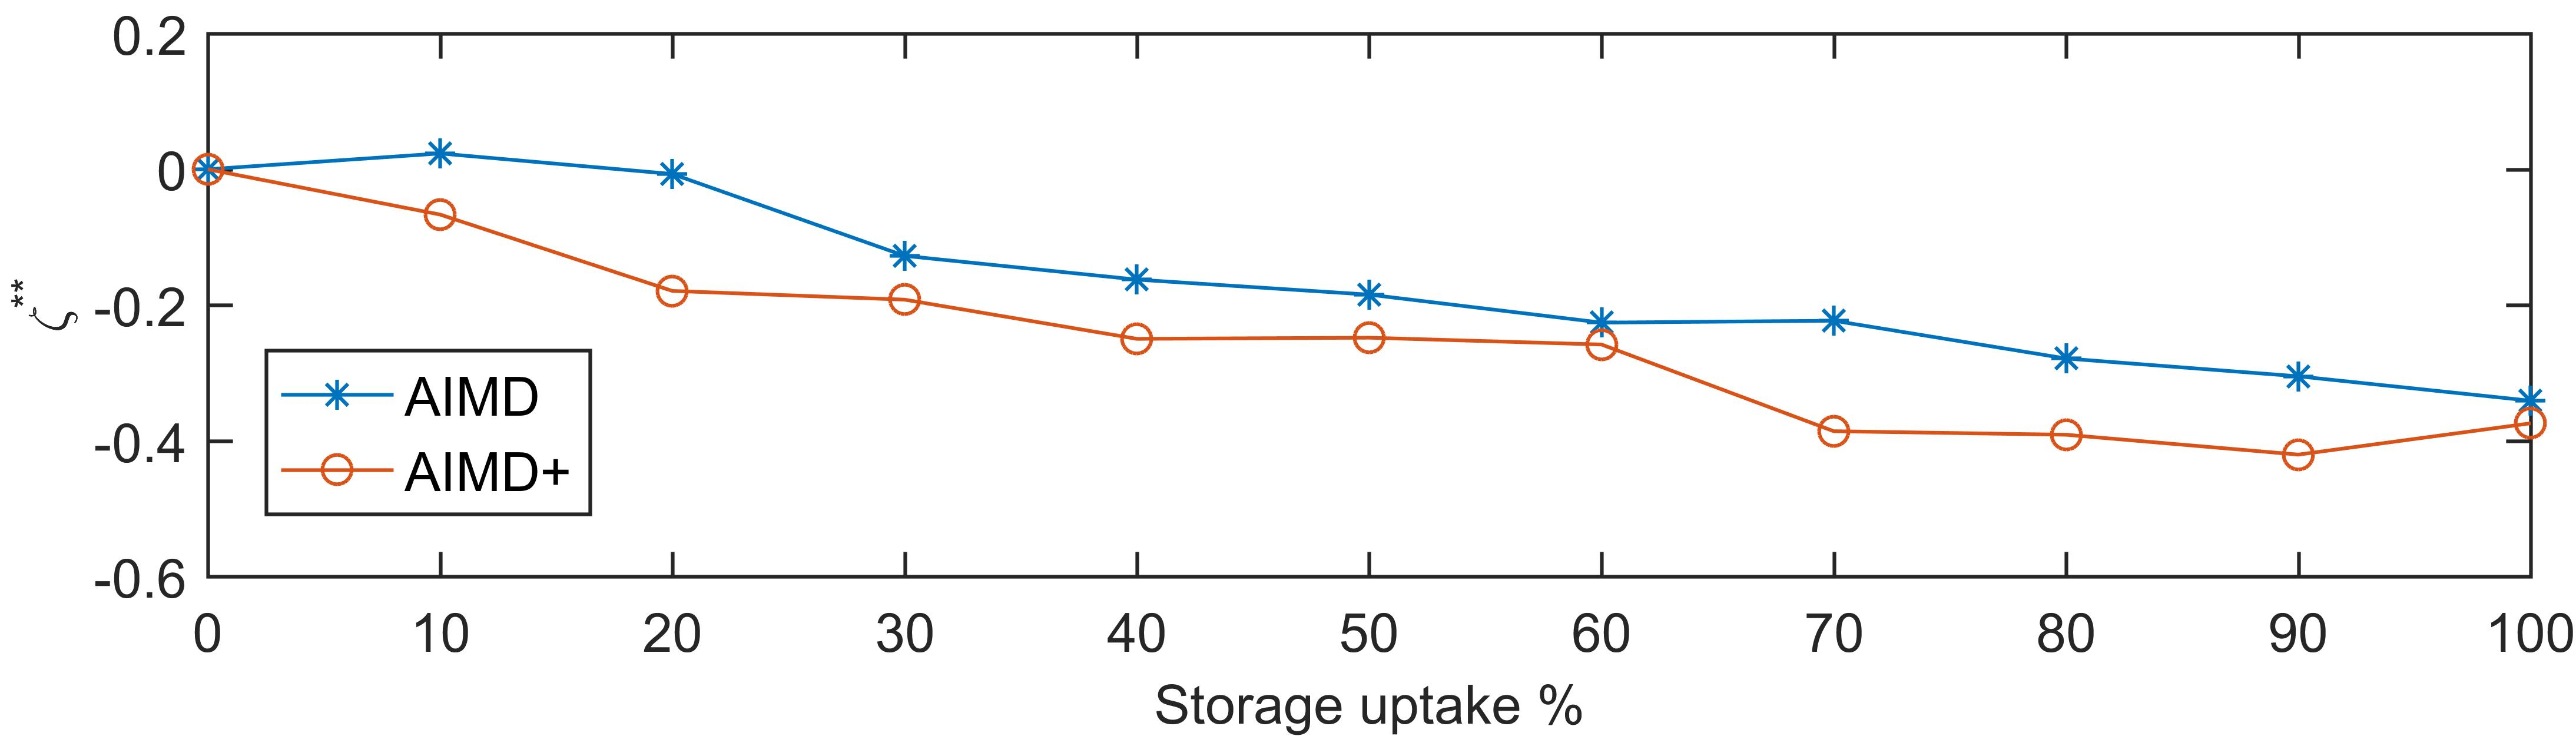
\includegraphics{_chapter1/fig/input/utilisation-AIMD-compare}
 \caption{Average $\zeta_\textbf{C}^{**}$ (AIMD) and $\zeta_\textbf{D}^{**}$ (AIMD+) values recorded against the corresponding storage~uptake.}
 \label{ch1:fig:utilisation-aimd-compare}
\end{figure}


Whilst the deployment of energy storage has often been seen as a possible solution to defer network reinforcements, the presented results show that this is not always the case. In fact, the importance of choosing an appropriate control algorithm outweighs the availability of the energy storage itself. This becomes particularly apparent when energy storage devices need to recharge their injected energy for times of peak demand. For the AIMD case, this recharging was not controlled sufficiently, which led to higher line currents. The proposed AIMD+ algorithm was not as susceptible to this kind of behaviour, as it has been designed to take battery location into account. This immunity and well-controlled power flow caused little to no additional strain on the network's equipment, allowing the deployed storage devices to also provide voltage support.

\subsection{Battery Utilisation Analysis}

In this part of the analysis, the batteries' fairness of usage was evaluated. The battery power profiles were recorded; excerpts are plotted in Figure \ref{ch1:fig:battery-utilisation-power} and are arranged by distance from the substation.

\begin{figure}[htb]\centering
 \subfloat[]{%
 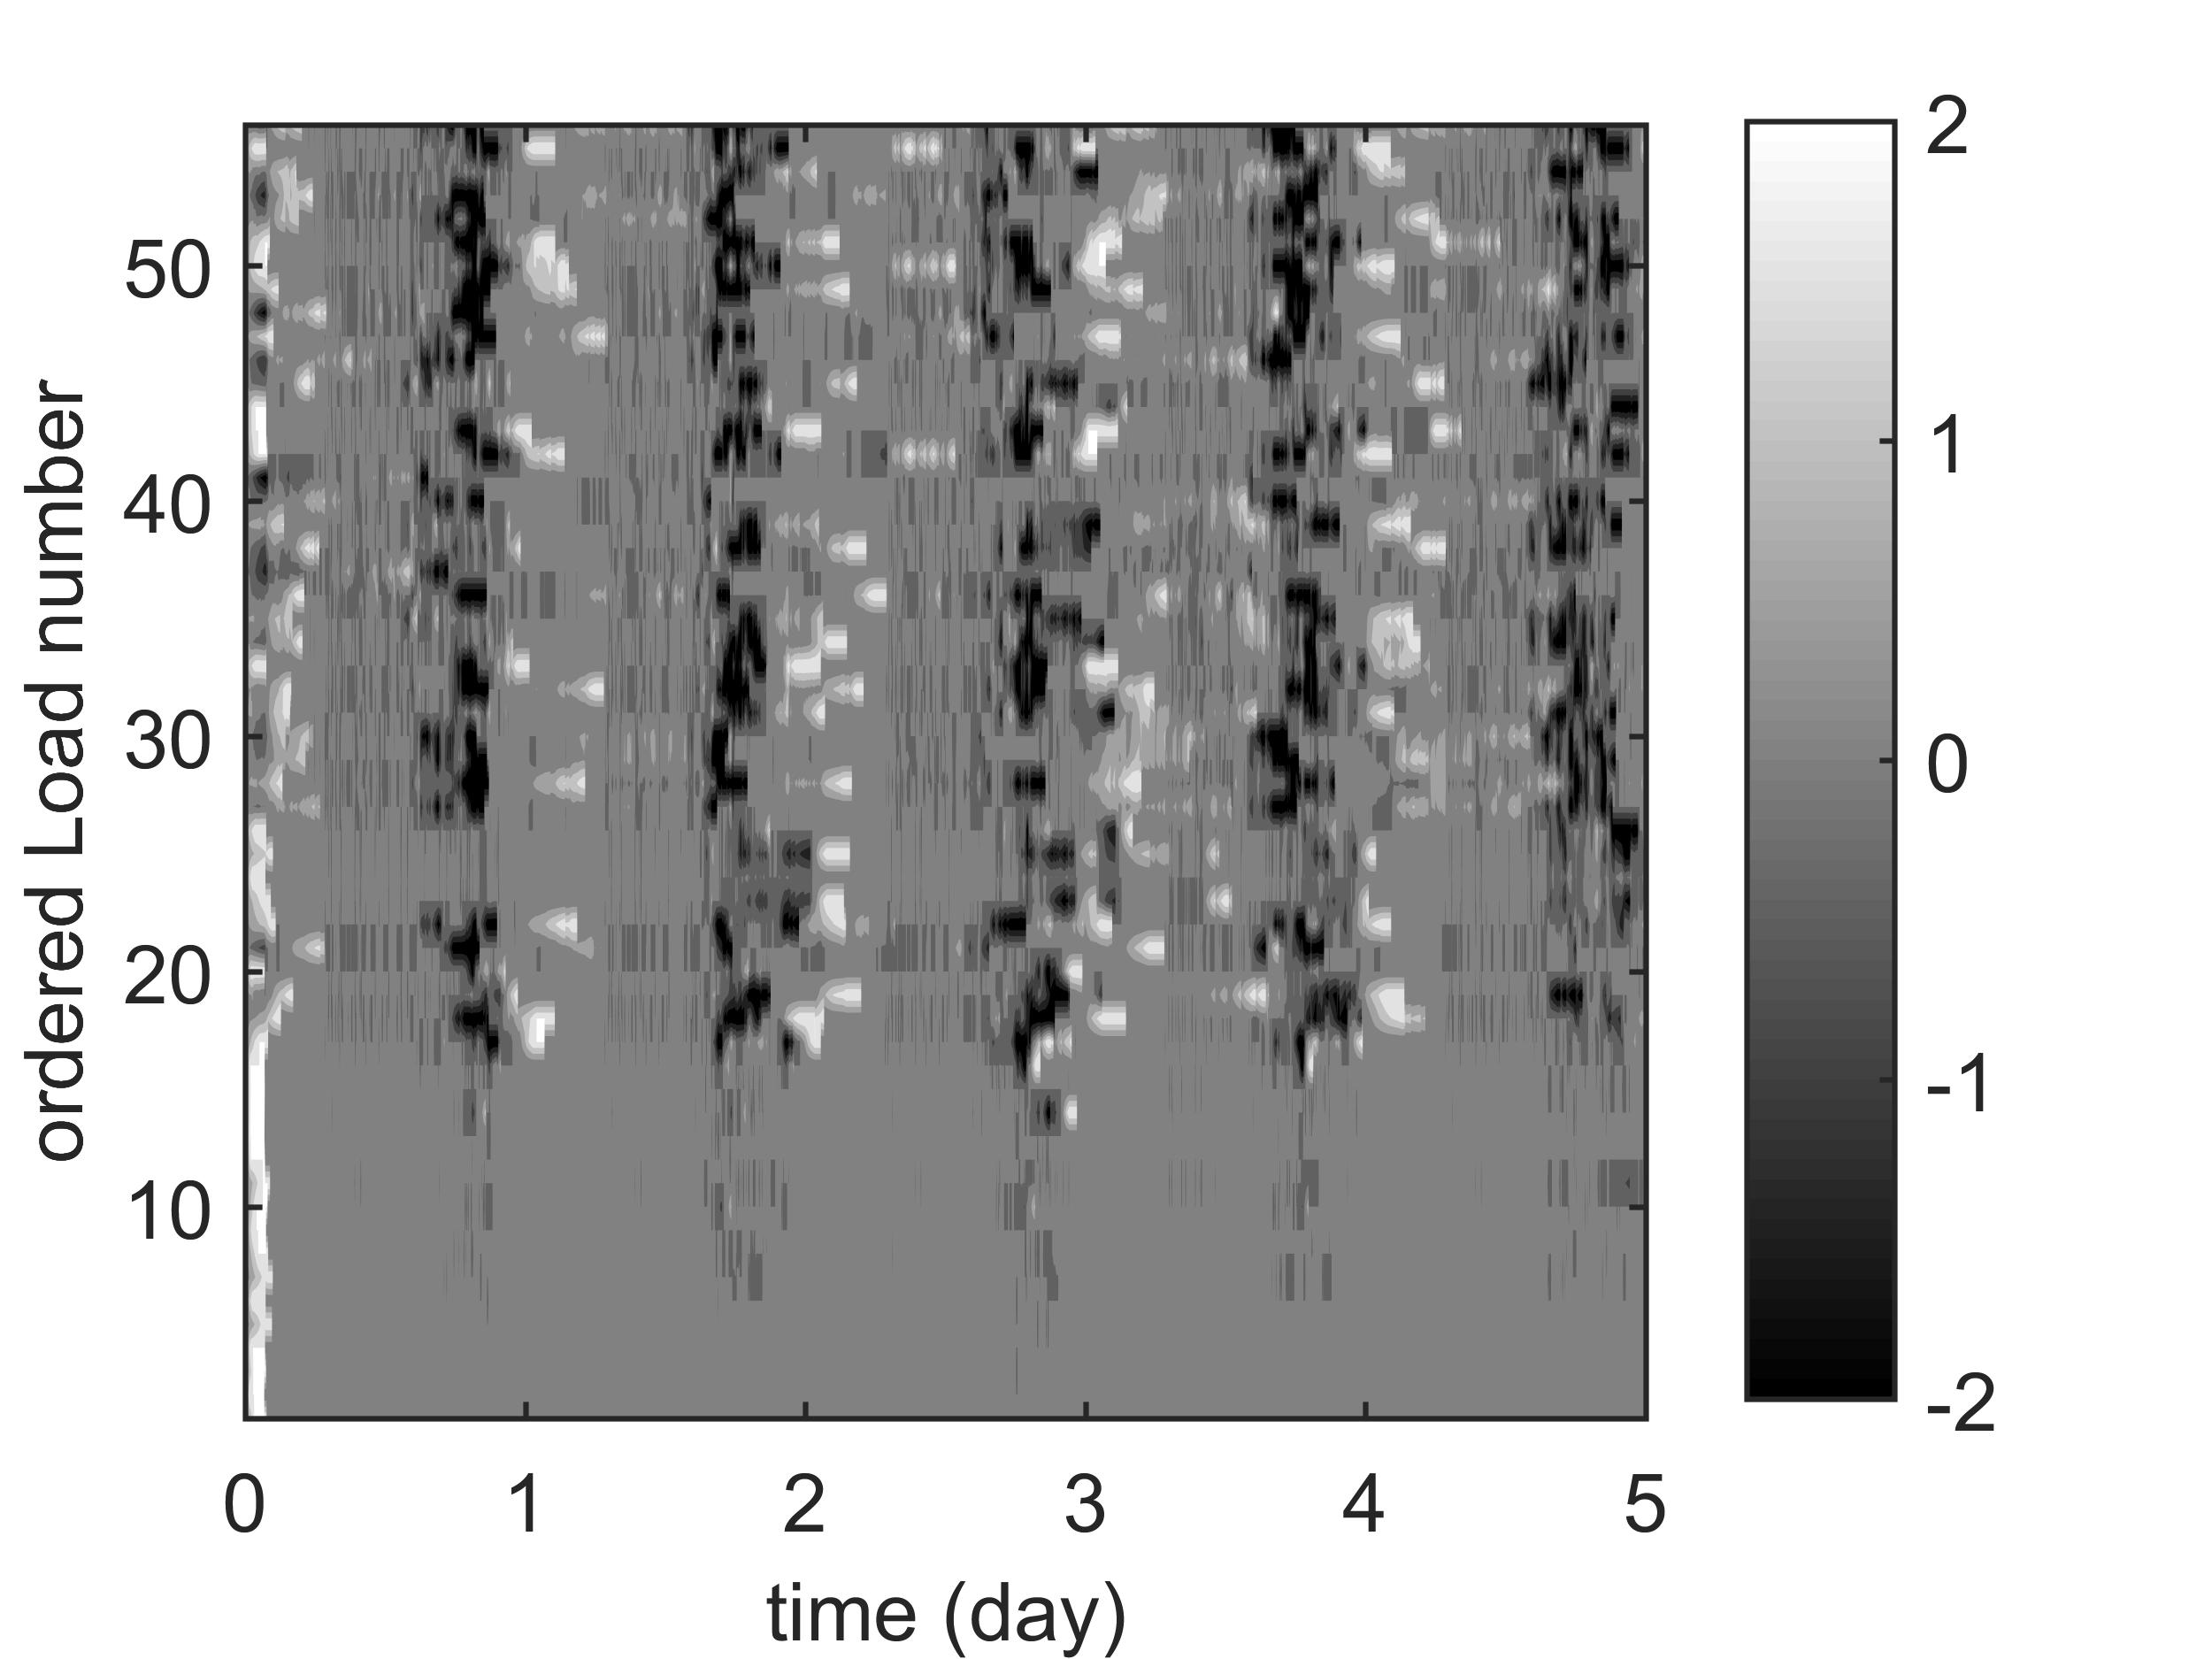
\includegraphics[width=0.48\textwidth]{_chapter1/fig/input/sorage-AIMD1-power}%
 \label{ch1:subfig:battery-utilisation-power-f}%
 }
 \subfloat[]{%
 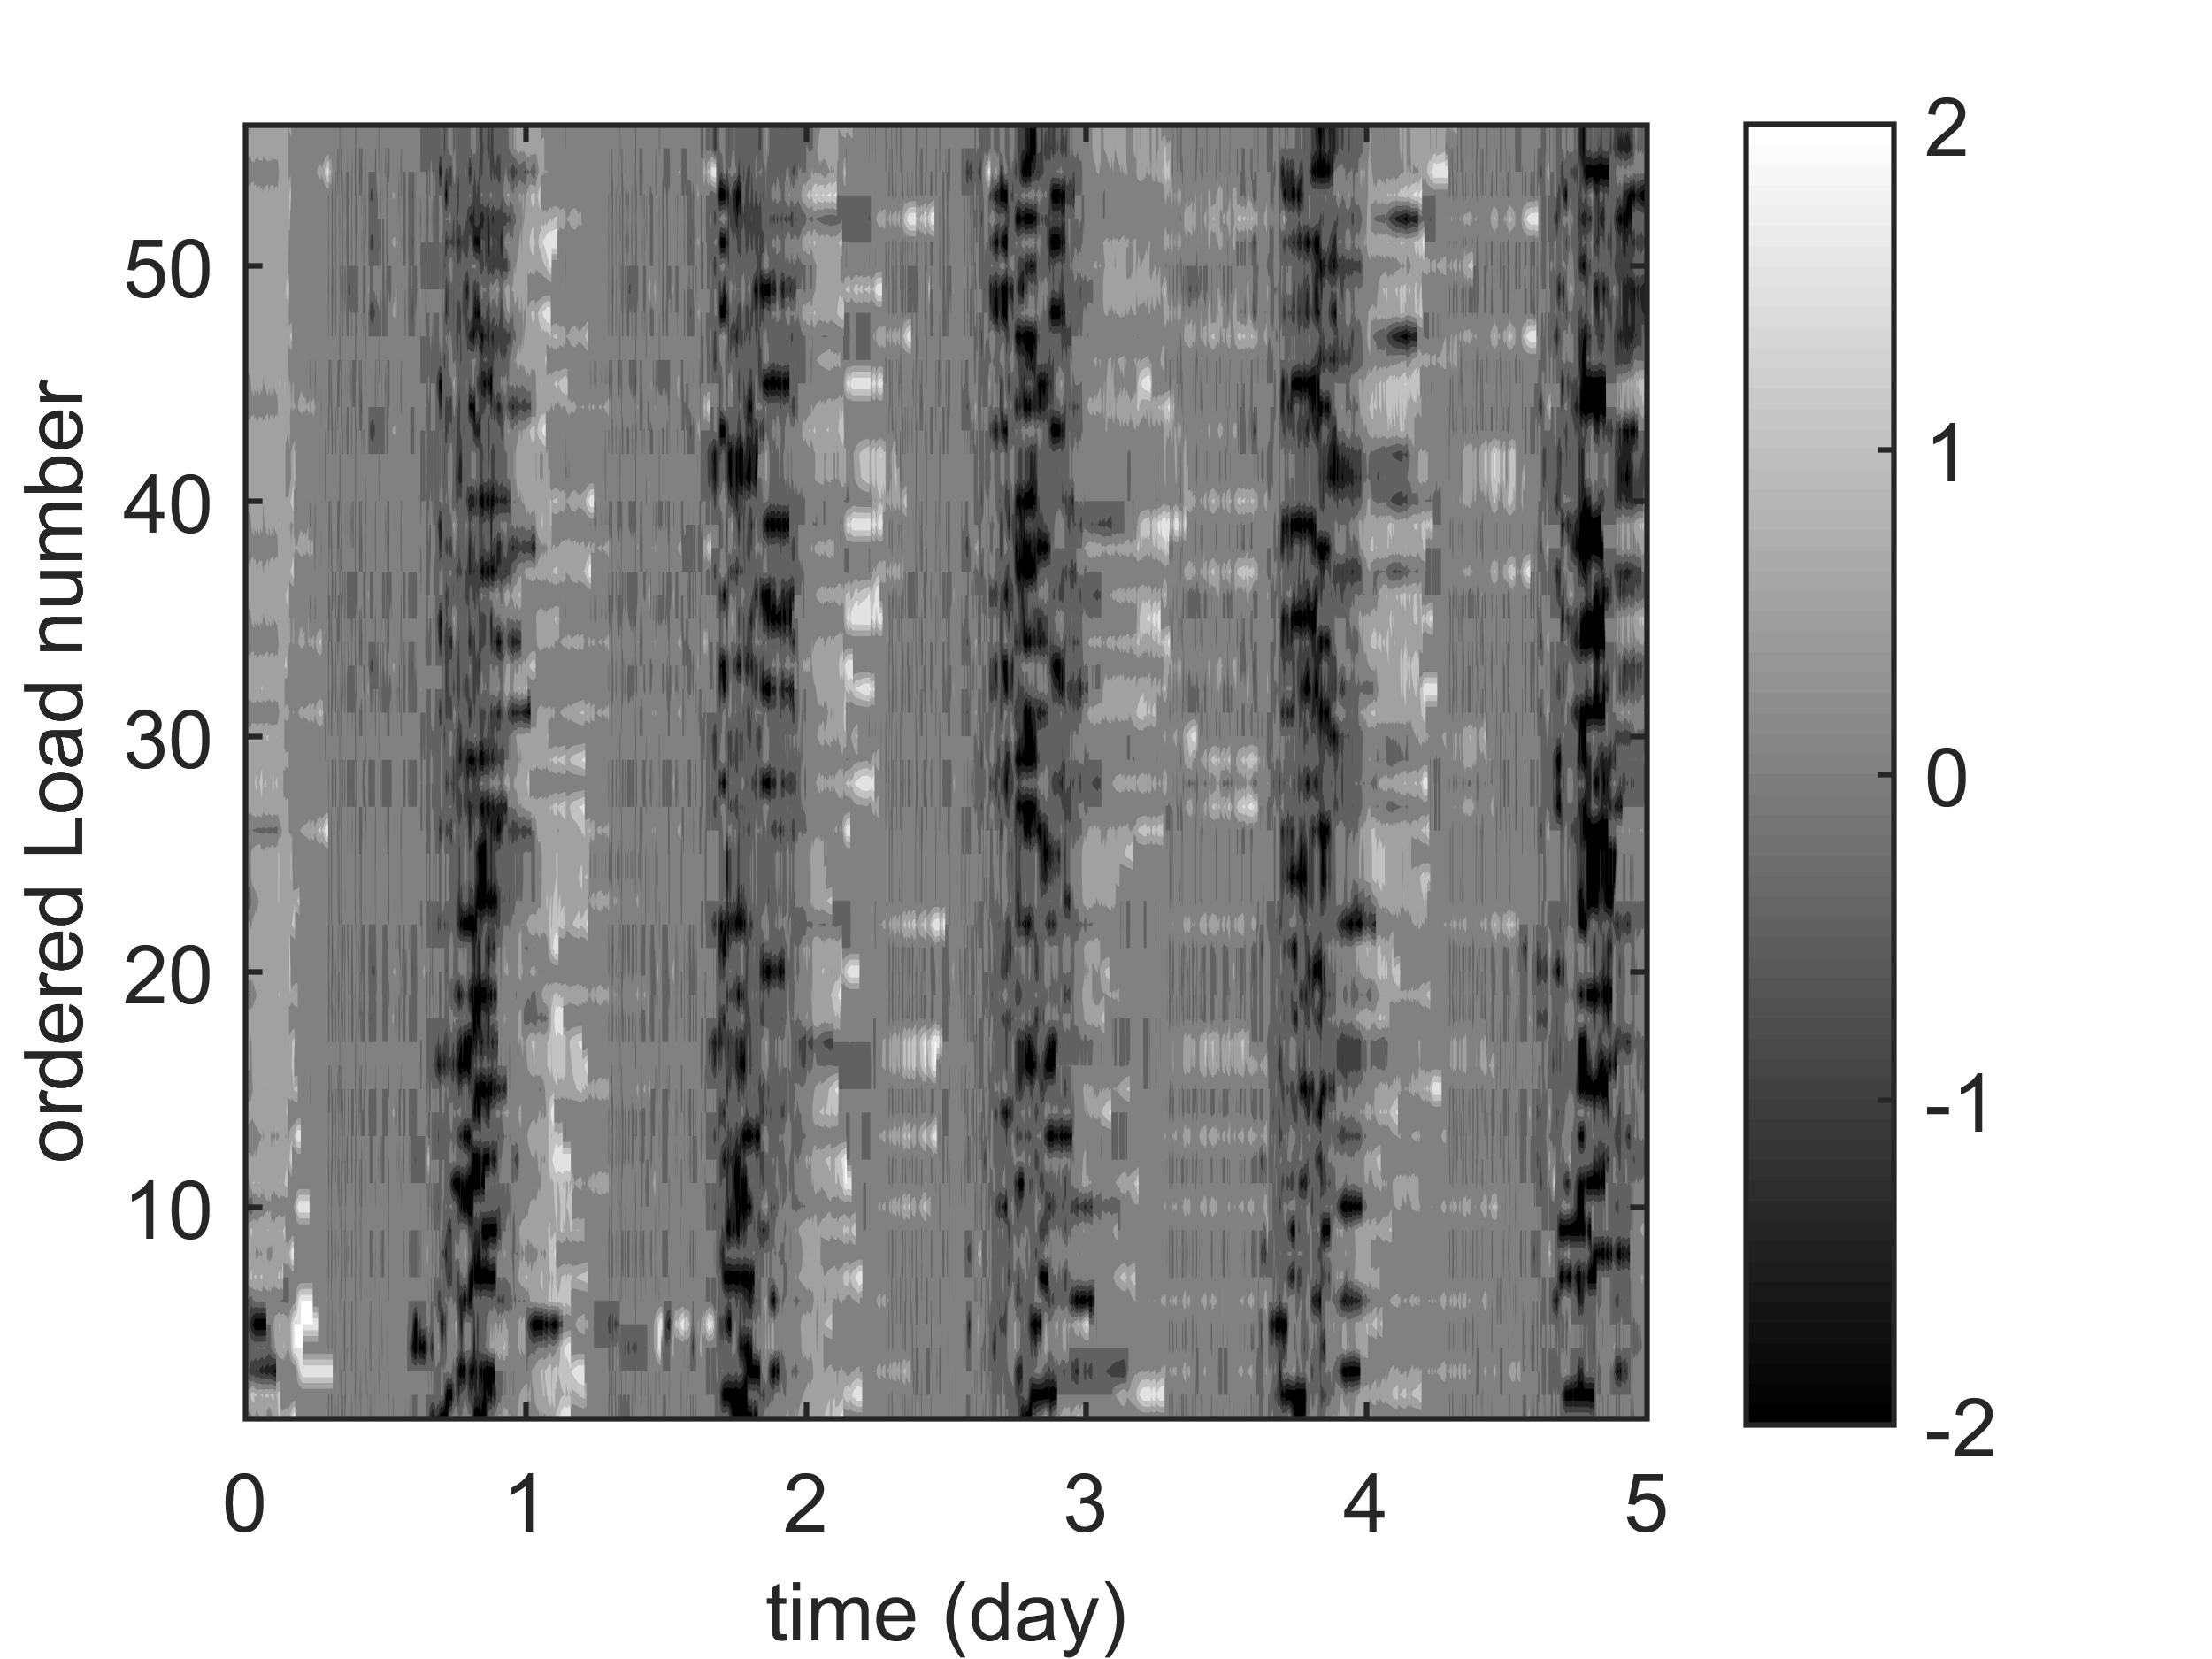
\includegraphics[width=0.48\textwidth]{_chapter1/fig/input/sorage-AIMD2-power}%
 \label{ch1:subfig:battery-utilisation-power-r}%
 }\vspace{-3pt}
 \caption{Battery power profiles of each load's battery storage device over four days for (\textbf{a}) AIMD  and (\textbf{b}) AIMD+. ({a}) Case {C}, 60\% EV and 100\% AIMD (kW); ({b}) Case {D}, 60\% EV and 100\% AIMD+ (kW).}
 \label{ch1:fig:battery-utilisation-power}
\end{figure}


In this figure, it can be seen that only half of the deployed storage devices were active in Case {C} (AIMD control), whereas all devices are utilised in Case {D} (AIMD+ control). From the recorded battery SOC profiles, the net cycling of each battery was computed and divided by the duration of the simulation, giving an average daily cycling value. This value is plotted for each load in Figure \ref{ch1:fig:battery-cycling}a. The corresponding statistical analysis is presented in Figure \ref{ch1:fig:battery-cycling}b.

\begin{figure}[!h]\centering
 \subfloat[]{%
 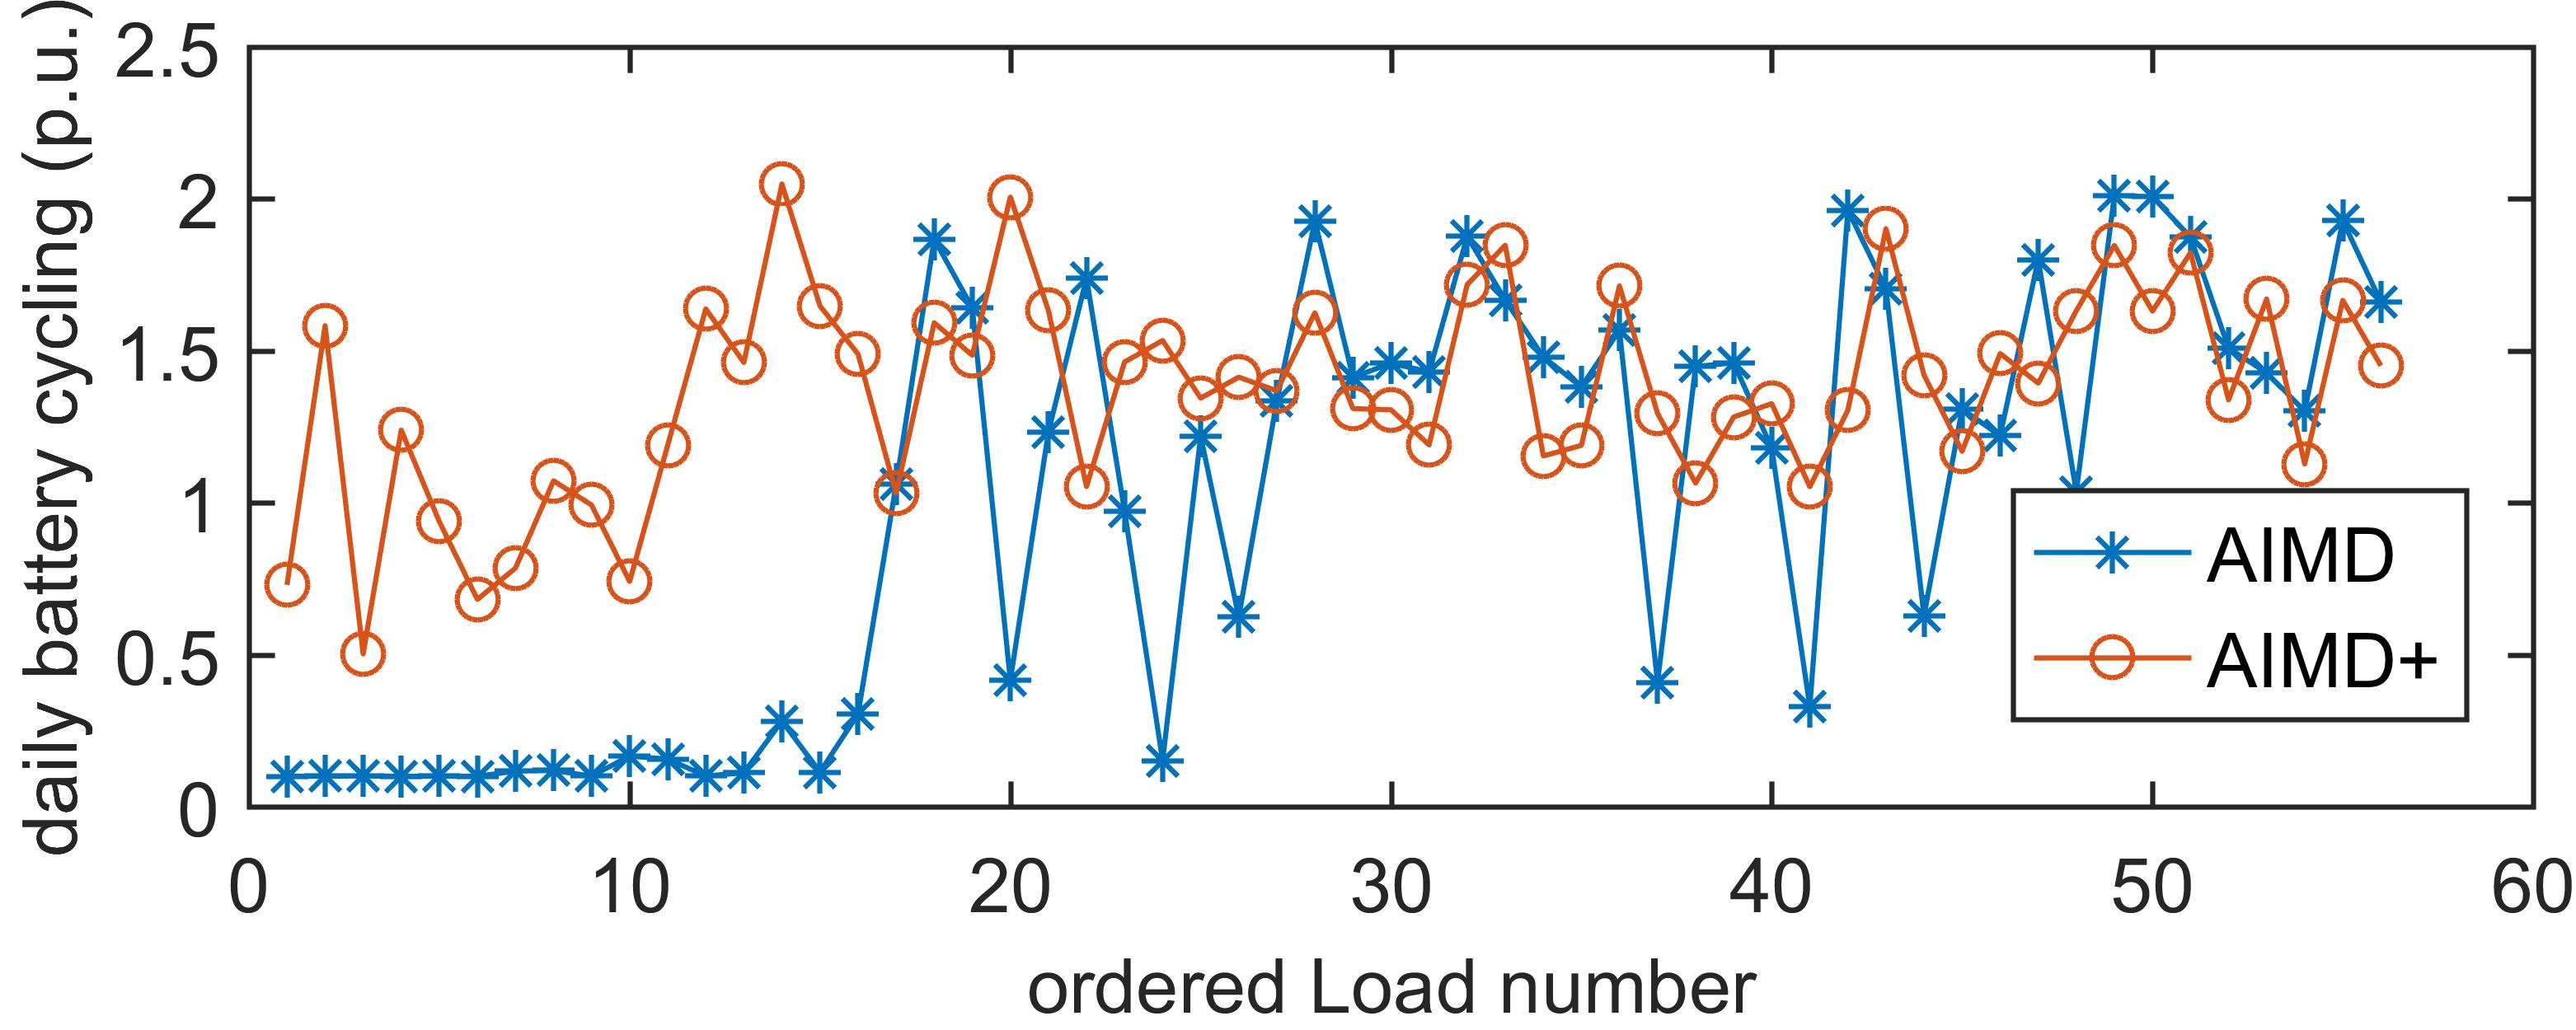
\includegraphics[height=0.25\textwidth]{_chapter1/fig/input/sorage-cycling-comparison}%
 \label{ch1:subfig:battery-cycling-excerpt}%
 }
 \hspace{5mm}
 \subfloat[]{%
 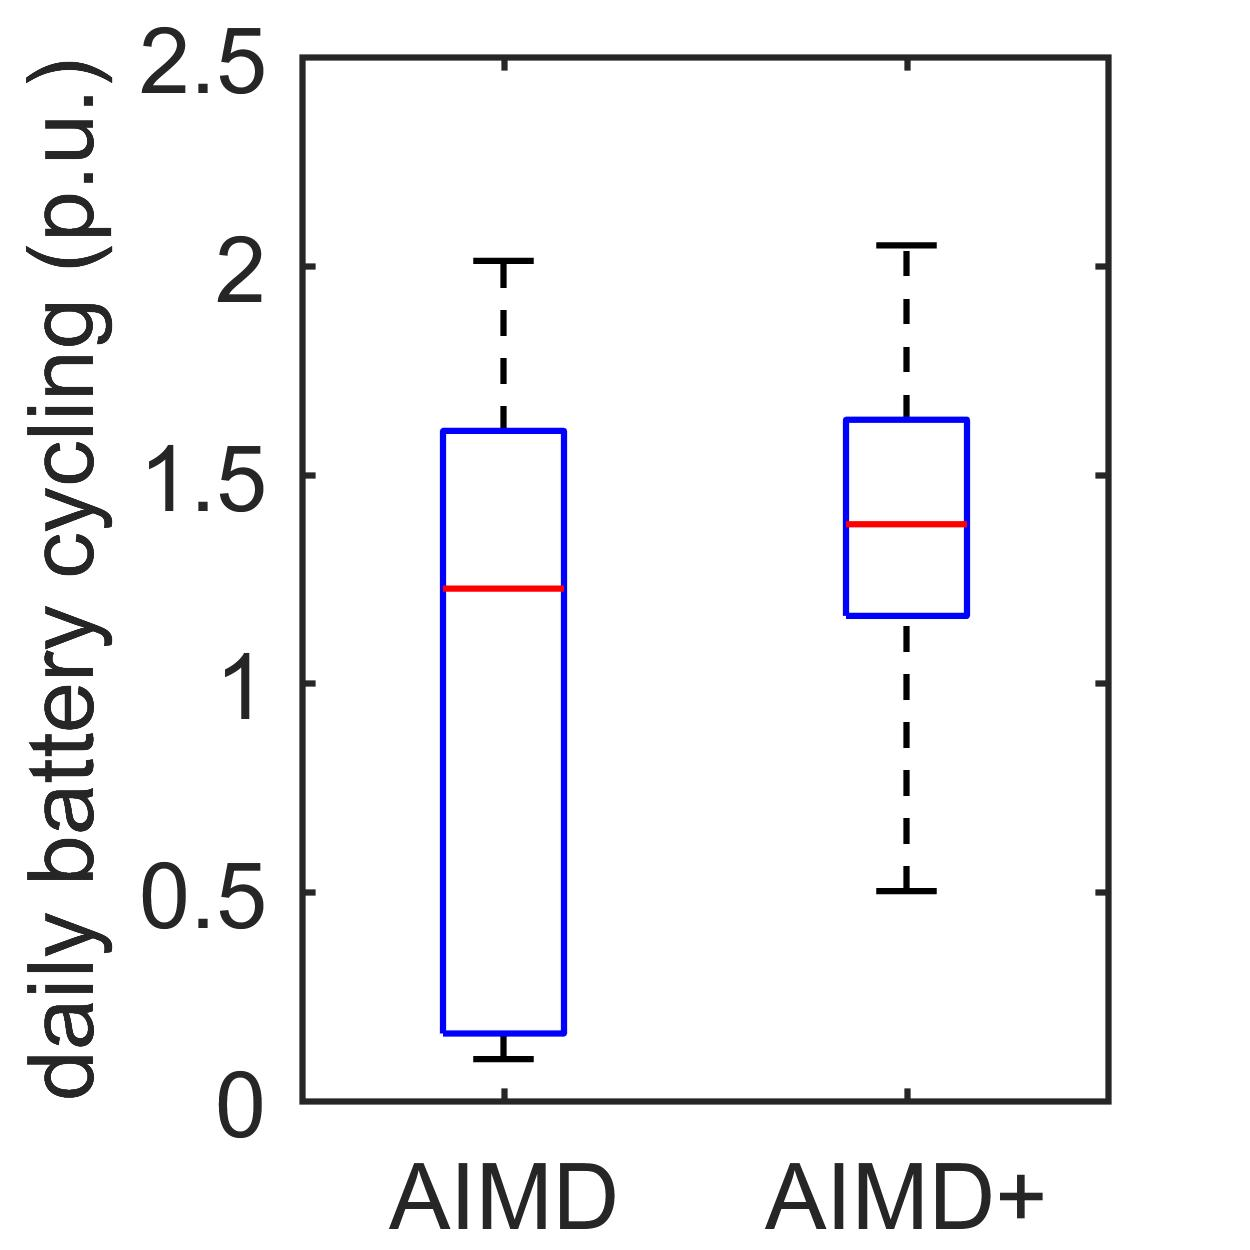
\includegraphics[height=0.25\textwidth]{_chapter1/fig/input/sorage-cycling-comparison-stats}%
 \label{ch1:subfig:battery-cycling-summary}%
 }
 \caption{Each load's battery cycling compared for (\textbf{a}) 60\% EV and 100\% AIMD and AIMD+ uptake  and (\textbf{b}) in a statistical context. Here, $\zeta_\textbf{C}^{***}=3.89$ and $\zeta_\textbf{D}^{***}=2.54$.}
 \label{ch1:fig:battery-cycling}
\end{figure}

These two plots show the under-usage of AIMD controlled batteries, as well as the variance in battery usage under AIMD and AIMD+ control. In fact, under AIMD control, 20 out of 55 batteries experienced a cycling of less than 10\% per day, whereas the remaining devices were utilised fully. This discrepancy causes the $\zeta_\textbf{C}^{***}$ value to be noticeably larger than $\zeta_\textbf{D}^{***}$. A more detailed comparison is given when plotting the Peak-to-Average Ratios (PAR) of the batteries' daily cycling over the full range of EV and storage uptake scenarios; these plots are shown in Figure \ref{ch1:fig:storage-par-large}. Section \ref{ch1:subsubsec:parameter-for-the-improvement-of-battery-cycling} gives the detail on the PAR, $\zeta^{***}$.

\begin{figure}[htb]\centering
 \subfloat[]{%
 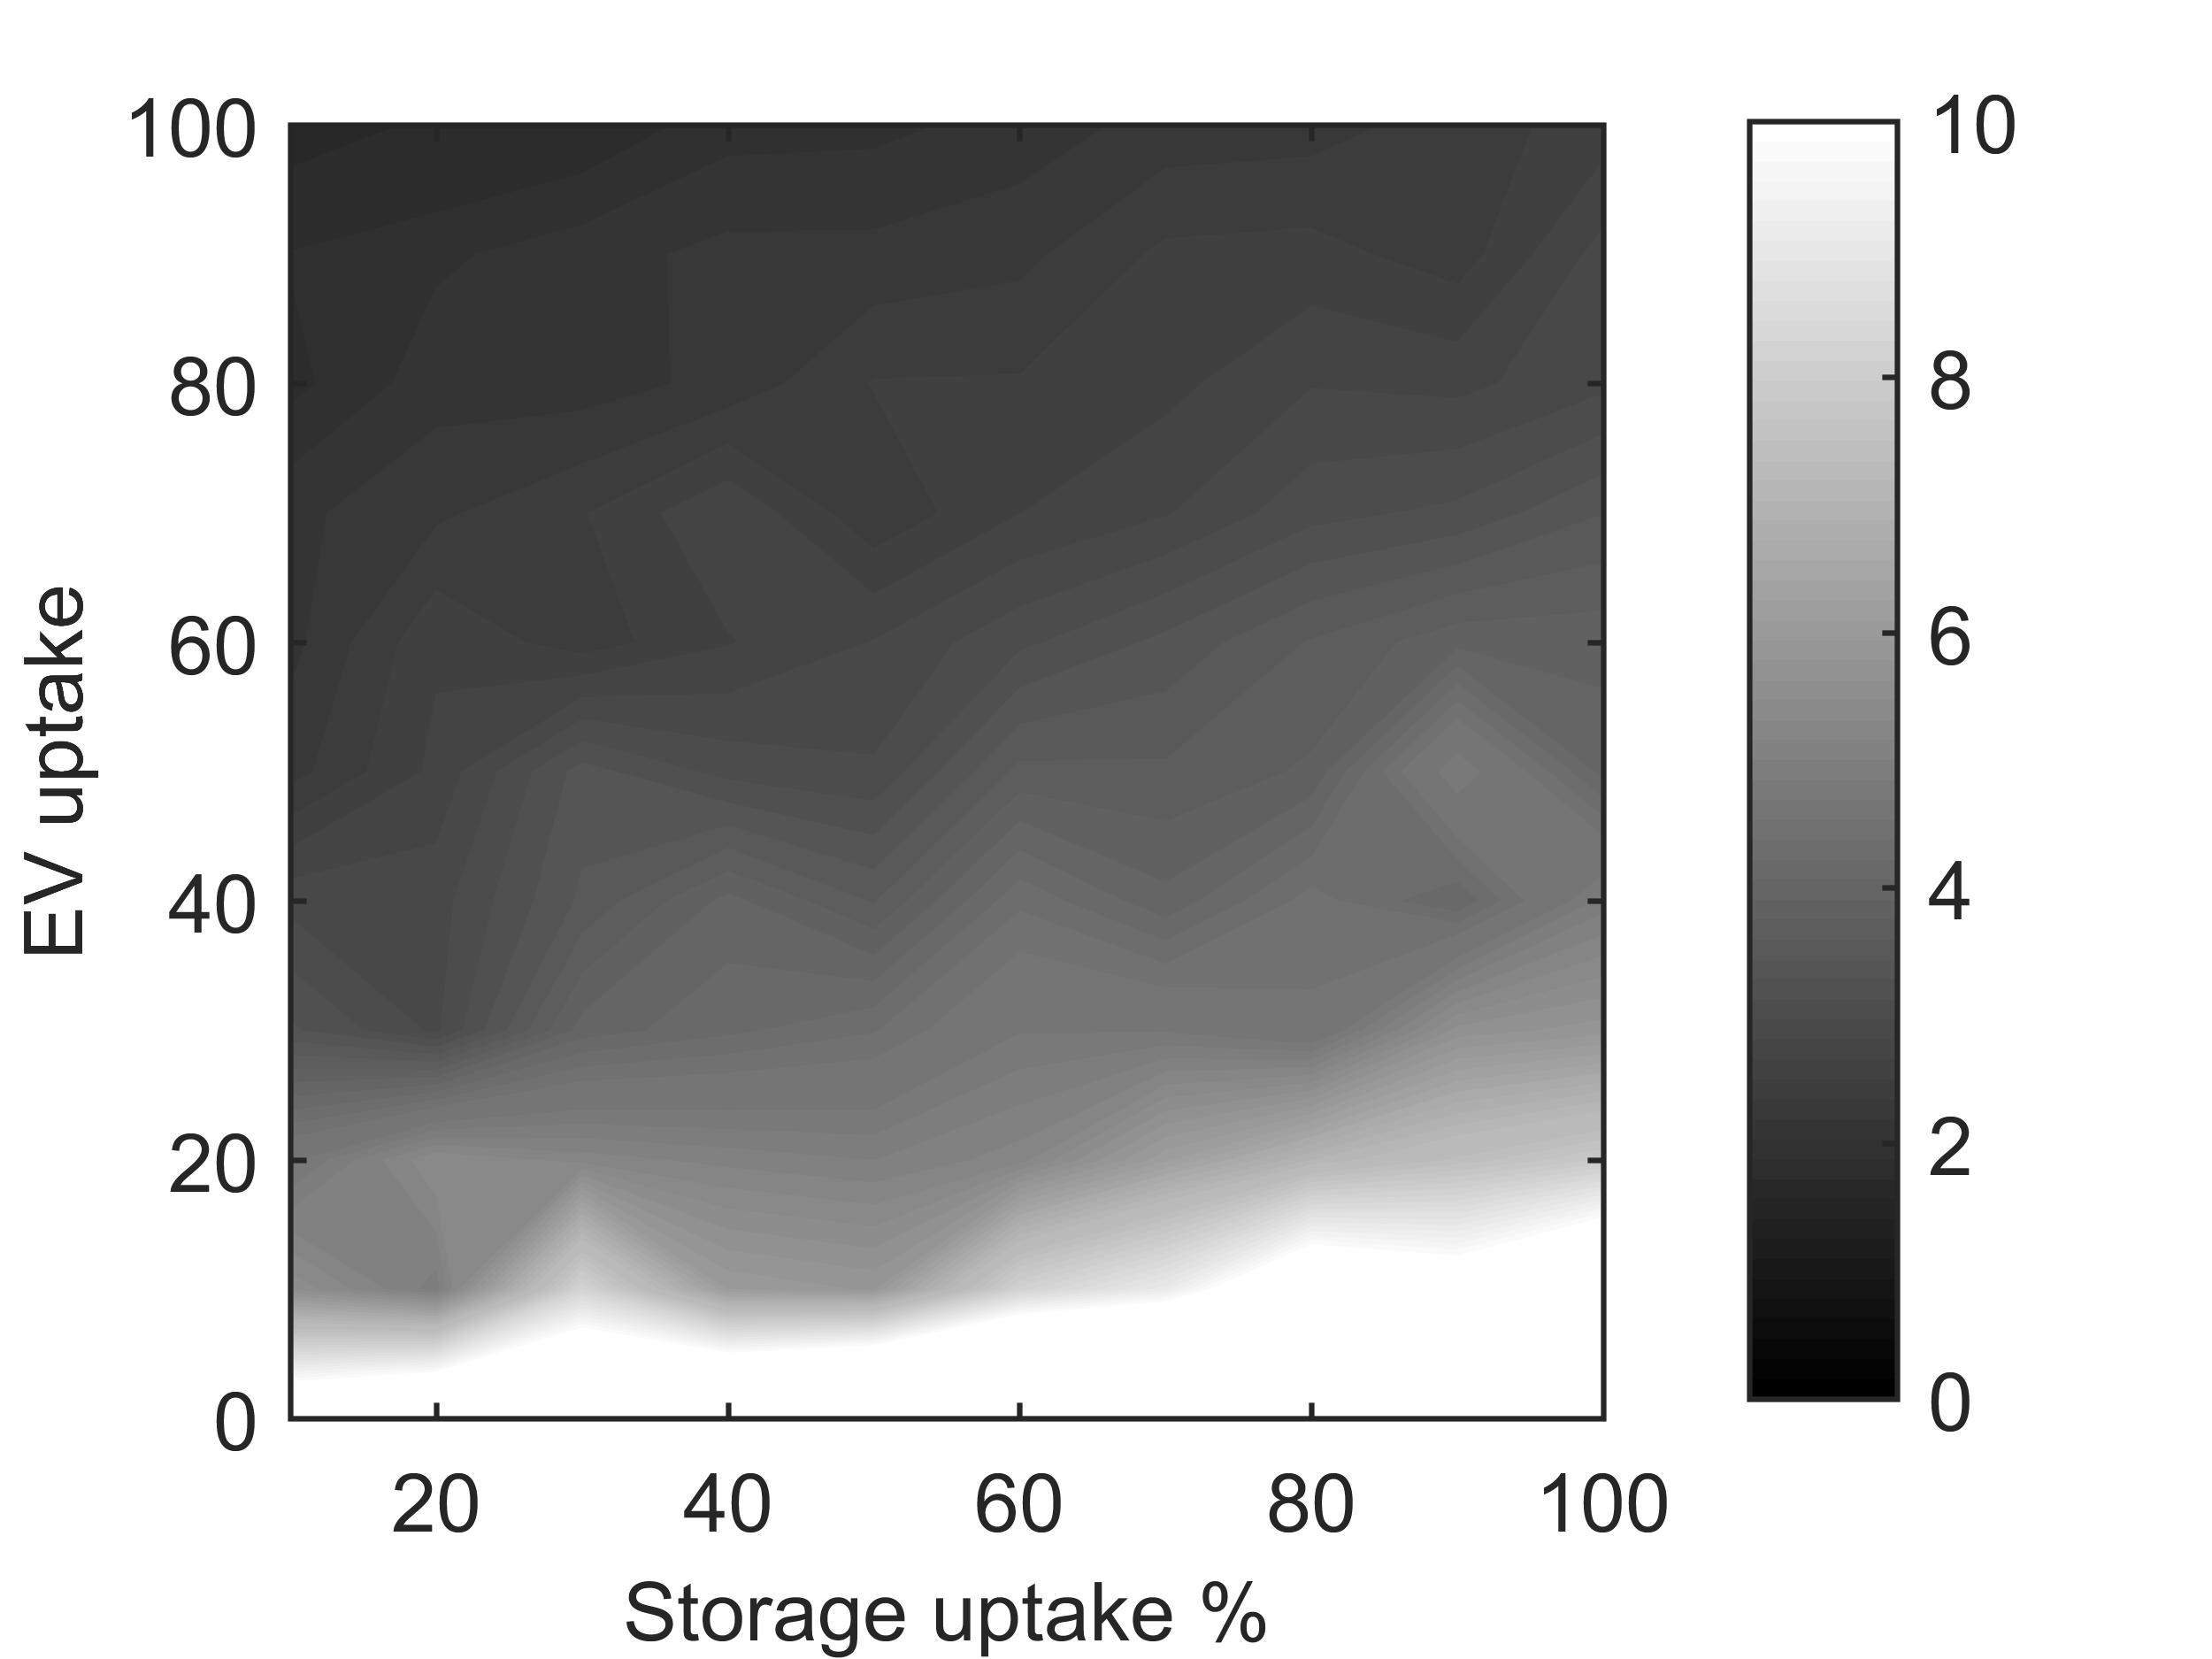
\includegraphics[width=0.48\textwidth]{_chapter1/fig/input/sorage-AIMD1-uptake-cycling-par}%
 \label{ch1:subfig:sotrage-AIMD1-uptake-cycling-par}%
 }
 \subfloat[]{%
 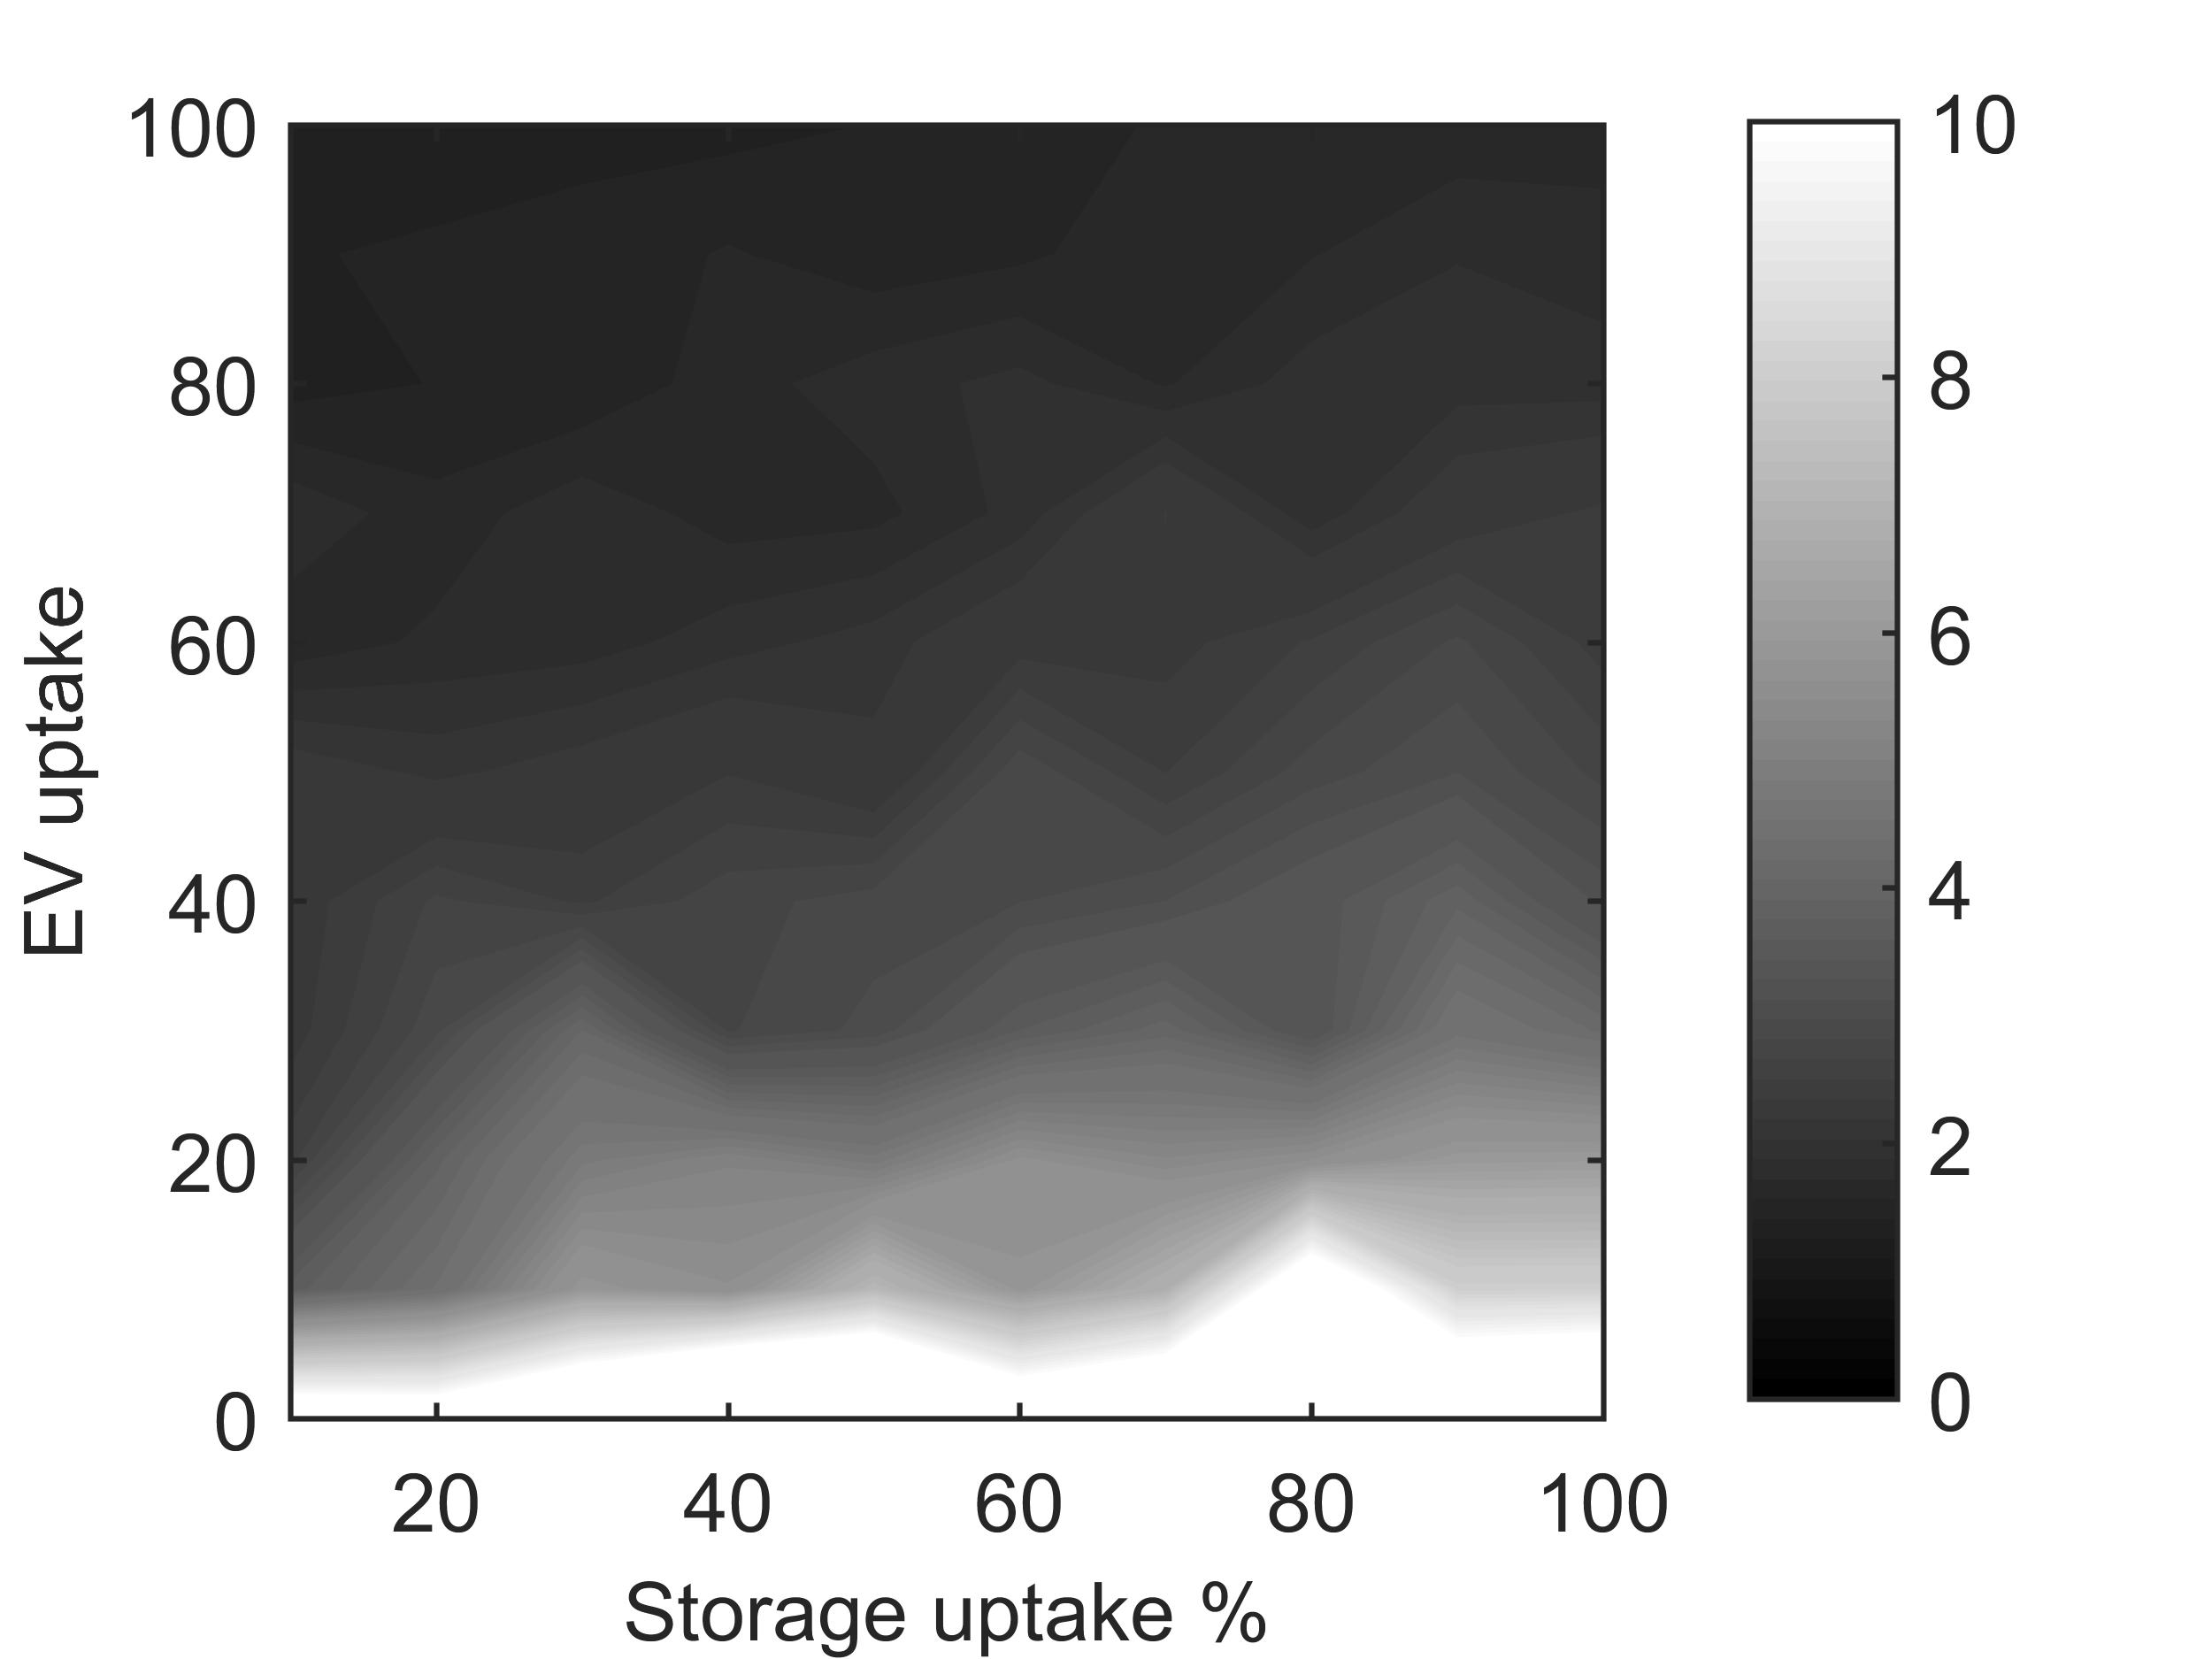
\includegraphics[width=0.48\textwidth]{_chapter1/fig/input/sorage-AIMD2-uptake-cycling-par}%
 \label{ch1:subfig:sotrage-AIMD2-uptake-cycling-par}%
 }\vspace{-6pt}
 \caption{Peak-to-Average Ratios (PAR) of the battery cycling profiles of each load's battery storage device over four days for (\textbf{a}) AIMD  and (\textbf{b}) AIMD+.}
 \label{ch1:fig:storage-par-large}
\end{figure}


The figure shows that for any EV uptake scenario, AIMD-controlled energy storage units were cycled less equally than the AIMD+ controlled devices. Results also show that with a low EV uptake, both the AIMD and AIMD+ algorithm performed worse; yet improved as EV uptake increased.

Averaging the PARs for all batteries' SOC profiles over all EV uptake percentages yields a clear performance difference between AIMD and AIMD+. These resulting PARs, i.e., the $\zeta_\textbf{C}^{***}$ and $\zeta_\textbf{D}^{***}$ values for their corresponding storage uptake percentages, are presented in Figure \ref{ch1:fig:storage-par}.

\begin{figure}[htb]\centering
 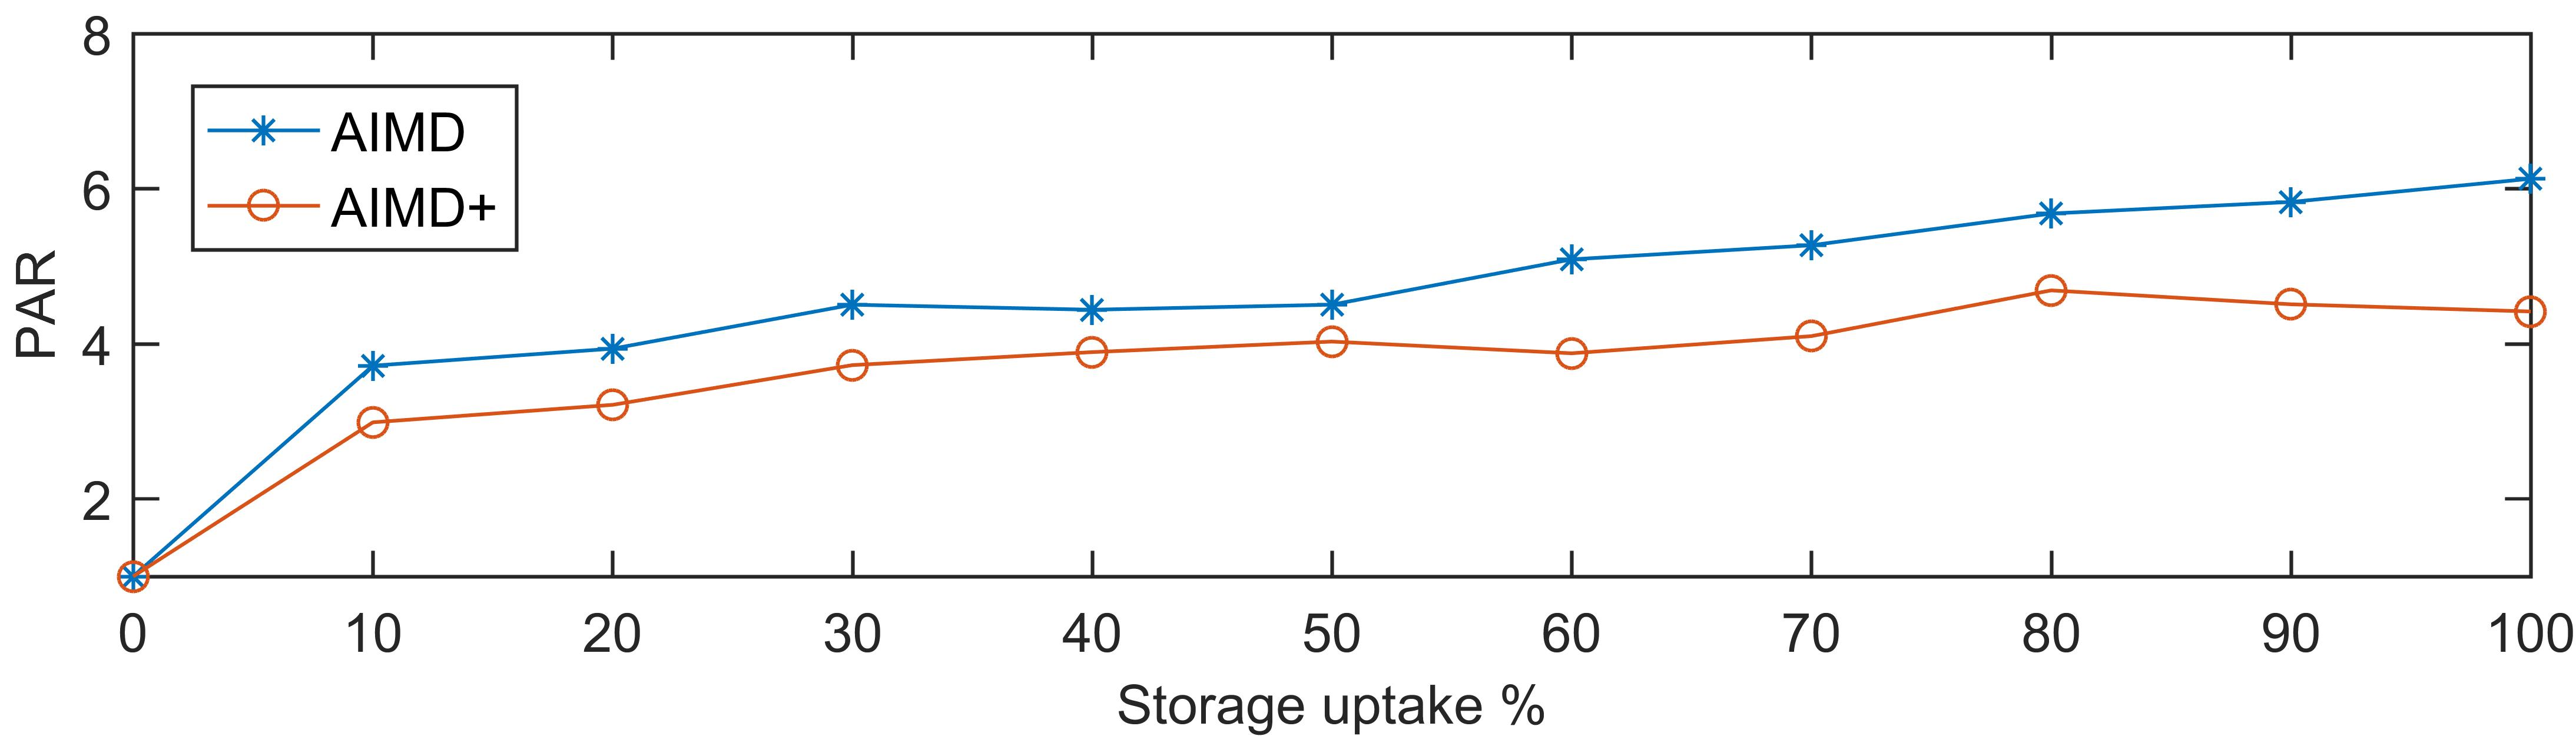
\includegraphics{_chapter1/fig/input/sorage-par}
 \caption{The performance index $\zeta_\textbf{C}^{***}$ for AIMD storage and $\zeta_\textbf{D}^{***}$ for AIMD+ storage control against storage uptake.}
 \label{ch1:fig:storage-par}
\end{figure}


Although the AIMD controlled batteries were, on average, cycled less than the batteries controlled by the proposed AIMD+ algorithm, looking at the average produces a distorted understanding of the performance. In fact, as more than half of the assigned AIMD BESS devices never partook in the network control, a lower average cycling was expected to begin with. The variation in cycling across all batteries, or the cycling PAR, reveals the difference between usage and effective usage. A lower ratio indicates a better usage of the deployed batteries.